\section{数学物理方程知识点}

\subsection{定解问题}

\subsubsection{边界条件的分类}
在数学上可归纳为以下 3 类边界条件:

(1) 第一类边界条件

在边界 $S$ 上给出未知函数 $ u $ 的取值, 即
$$
\left.u\right|_{S}=f_{1}
$$
这种形式的边界条件称为第一类边界条件. 弦振动问题中的固定端即满足第一类边界条件或狄利克雷(Dirichlet)条件.

(2) 第二类边界条件

在边界 $ S $ 上给出未知函数 $ u $ 沿 $ S $ 的外法线方向的方向导数, 即
$$
\left.\frac{\partial u}{\partial n}\right|_{S}=f_{2}
$$
这种形式的边界条件称为第二类边界条件或纽曼 (Neumann)条件. 在热传导问题中, 在边界处绝热即属于第二类边界条件.

(3) 第三类边界条件

在边界 $S$ 上给出未知函数 $u$ 及其沿 $S$ 的外法线方向的方向导数某种线性组合的值, 即
$$
\left.\left(\frac{\partial u}{\partial n}+\sigma u\right)\right|_{S}=f_{3}
$$
这种形式的边界条件属于第三类边界条件或罗宾(Robin)条件. 弦振动问题中的弹性支承端即满足第三类边界条件.

上述问题中的 $ f_{i}(i=1,2,3) $ 是定义在边界 $ S $ 上的已知函数. 当 $ f_{i} \equiv 0 $ 时,相应的边界条件为齐次的, 当 $ f_{i} \neq 0 $ 时, 相应的边界条件为非齐次的.

\subsubsection{定解问题}

描写一个物理过程的方程称为泛定方程. 初始条件和边界条件总称为定解条件. 泛定方程带上适当的定解条件, 就构成了数学物理中的定解问题. 下面讨论 3 类方程常见定解问题的提法.

由泛定方程和初始条件构成的定解问题称为初始问题(或柯西(Canchy)问题).\\
例如一条想象中的无限长的弦的自由振动问题可表示为如下柯西问题:
$$
\left\{\begin{array}{l}
u_{t t}=a^{2} u_{x x} \quad-\infty < x < +\infty, t >0 \\
\left.u\right|_{t=0}=\varphi(x) \\
\left.u_{t}\right|_{t=0}=\psi(x)
\end{array}\right.
$$
理想中无限长的杆的热传导问题可表示为如下的柯西问题:
$$
\left\{\begin{array}{l}
u_{t}=a^{2} u_{x x} \quad-\infty< x < +\infty, t>0 \\
\left.u\right|_{t=0}=\varphi(x)
\end{array}\right.
$$

泛定方程和边界条件构成的定解问题称为边值问题. 拉普拉斯方程和泊松方程与时间 $ t $ 无关, 所以不能提初始条件, 因此这两类方程相应的定解问题只有边值问题. 因为边界条件有 3 类,所以拉普拉斯方程(调和方程)的边值问题有 3 种.

(1) 第一边值问题

拉氏方程与第一边界条件组成的定解问题称为第一边值问题, 也称为狄利克雷(Dirichlet) 问题. 例如:
$$
\left\{\begin{array}{cc}
\Delta_{3} u=f(x, y, z) & (x, y, z) \in \Omega \\
\left.u\right|_{\partial \Omega}=\varphi(x, y, z) & (x, y, z) \in \partial \Omega
\end{array}\right.
$$
(2) 第二边值问题

拉氏方程与第二边界条件组成的定解问题称为第二边值问题,也称为纽曼 (Neumann) 问题. 例如:
$$
\left\{\begin{array}{cc}
\Delta_{3} u=f(x, y, z) & (x, y, z) \in \Omega \\
\left.\frac{\partial u}{\partial n}\right|_{\partial \Omega}=\varphi(x, y, z) & (x, y, z) \in \partial \Omega
\end{array}\right.
$$
(3) 第三边值问题

拉氏方程与第三边界条件组成的定解问题称为第三边值问题, 也称为洛平 (Robin) 问题. 例如:
$$
\left\{\begin{array}{l}
\Delta_{3} u=f(x, y, z),(x, y, z) \in \Omega \\
\left.\left(\frac{\partial u}{\partial n}+\sigma u\right)\right|_{\partial \Omega}=\varphi(x, y, z)
\end{array}\right.
$$

既有初始条件又有边界条件的定解问题称为混合问题. 例如:
$$
\left\{\begin{array}{ll}
u_{t t}=a^{2} u_{x x} & 0 < x < l,  t > 0 \\
\left.u\right|_{t=0}=\varphi(x),\left.u_{t}\right|_{t=0}=\psi(x) & 0 < x < l \\
\left.u\right|_{x=0}=0,\left.u\right|_{x=l}=0 & t>0
\end{array}\right.
$$
即为弦振动方程的混合问题.

\subsection{定解问题的适定性}
如果一个定解问题的解存在、唯一且稳定, 就称这个定解问题是适定的; 反之,若有一个性质不满足,则称这个定解问题是不适定的.

所谓解存在, 是指定解问题至少有一个解. 如果一个定解问题的解不存在,这个问题就完全失去了意义, 但定解问题反映的是客观物理实际, 在实际问题中解是存在的. 若定解问题的解不存在, 说明所建立的定解问题是错误的, 可能在推导过程中有非次要因素被忽略掉了, 导致泛定方程错误,还有可能定解条件给错了等. 这就需要重新考虑定解问题的提法.

解的唯一性从物理学上讲是显然的, 如果解存在但不唯一, 将无法确定所求解是否是所需要的, 当然也无法求近似解. 这表明问题的提法还不够确切, 需要进一步分析.

所谓解的稳定性, 是指当定解条件有微小变动时, 解是否相应地有微小的变动, 如果是这样, 该解就是稳定的解; 否则所得的解就没有实用价值, 因为定解条件通常是利用实验方法获得的, 因而所得到的结果总有一定的误差, 如果因此导致解的变动很大,那么这种解显然不符合客观实际的要求.

\subsection{分离变量法}
\subsubsection{有界弦的自由振动问题}
考察两端固定的弦的自由振动问题:
$$
\left.\left\{\begin{array}{ll}u_{tt}=a^2u_{xx}(0<x<l,t>0)&(1)\\u(0,t)=0,u(l,t)=0&(2)\\u(x,0)=\varphi(x),u_t(x,0)=\psi(x)&(3)\end{array}\right.\right.
$$
这个定解问题的特点是: 方程是线性齐次的, 边界条件也是线性齐次的. 像这种问题可以直接使用叠加原理, 即先寻求方程 (1) 满足边界条件 (2) 的足够多的特解, 再利用它们做线性组合, 使其满足初始条件 (3). 下面分 4 步介绍上述定解问题的求解.

\textbf{1. 分离变量}

设方程 (1) 有形如 $ u(x, t)=X(x) T(t) $ 的非零特解, 代人方程 (1), 得
$$
X(x) T^{\prime \prime}(t)=a^{2} T(t) X^{\prime \prime}(x)
$$
即
$$
\frac{X^{\prime \prime}(x)}{X(x)}=\frac{T^{\prime \prime}(t)}{a^{2} T(t)}
$$
上式左边是 $ x $ 的函数, 与 $ t $ 无关, 右边是 $ t $ 的函数, 与 $ x $ 无关. 要使上式成立, 只能使它们等于同一个常数. 记此常数为 $ -\lambda $, 于是得到 $ X(x) $ 与 $ T(t) $ 分别满足的常微分方程:
$$
\begin{array}{c}
X^{\prime \prime}(x)+\lambda X(x)=0 \quad(4)\\
T^{\prime \prime}(t)+\lambda a^{2} T(t)=0\quad(5)
\end{array}
$$
同样, 将 $ u(x, t) $ 代人边界条件 (2), 得
$$
X(0) T(t)=0, X(l) T(t)=0
$$
因为 $ T(t) $ 不能恒为 0 ,所以从上式可以得到
$$
X(0)=0, X(l)=0
$$

\textbf{2. 本征值问题的求解}

通过上面的变量分离得到 $ X(x) $ 满足的边值问题是
$$
\left\{\begin{array}{l}
X^{\prime \prime}(x)+\lambda X(x)=0 \quad(4)\\
X(0)=0, X(l)=0\quad(6)
\end{array}\right.
$$
这里的 $ \lambda $ 是待定的常数, 既要求出非零解 $ X(x) $, 又要定出常数 $ \lambda $, 这种常微分方程的边值问题称为本征值问题, $ \lambda $ 称为本征值, $ X(x) $ 称为本征函数. 下面求解本征值问题. 对 $ \lambda $ 的取值分 3 种情况进行讨论.

(1) 当 $ \lambda<0 $ 时,方程 (4) 的通解为
$$
X(x)=C_{1} \mathrm{e}^{\sqrt{-\lambda} x}+C_{2} \mathrm{e}^{-\sqrt{-\lambda} x}
$$
代人到要满足的边值条件 (6), 得
$$
\left\{\begin{array}{l}
C_{1}+C_{2}=0, \\
C_{1} \mathrm{e}^{\sqrt{-\lambda} l}+C_{2} \mathrm{e}^{-\sqrt{-\lambda} l}=0
\end{array}\right.
$$
因为此方程组的系数行列式
$$
\left|\begin{array}{cc}
1 & 1 \\
\mathrm{e}^{\sqrt{-\lambda} l} & \mathrm{e}^{-\sqrt{-\lambda} l}
\end{array}\right|=\mathrm{e}^{-\sqrt{-\lambda} l}-\mathrm{e}^{\sqrt{-\lambda} l} \neq 0
$$
所以该方程组有唯一的零解, $ C_{1}=C_{2}=0 $, 从而 $ X(x) \equiv 0 $, 不符合非零解的要求.

(2) 当 $ \lambda=0 $ 时,方程 (4) 的通解为
$$
X(x)=C_{1} x+C_{2}
$$
代人到边值条件 (6), 得
$$
\left\{\begin{array}{l}
C_{2}=0 \\
C_{1} l+C_{2}=0
\end{array}\right.
$$
故 $ C_{1}=C_{2}=0 $, 从而 $ X(x) \equiv 0 $, 不符合非零解的要求.

(3) 当 $ \lambda>0 $ 时,方程 (4) 的通解为
$$
X(x)=C_{1} \cos \sqrt{\lambda} x+C_{2} \sin \sqrt{\lambda} x
$$
代人到边值条件(6), 得
$$
\left\{\begin{array}{l}
C_{1}=0 \\
C_{1} \cos \sqrt{\lambda} l+C_{2} \sin \sqrt{\lambda} l=0
\end{array}\right.
$$
故 $ C_{2} \sin \sqrt{\lambda} l=0 $, 要求 $ X(x) \neq 0 $, 必须有 $ C_{2} \neq 0 $, 于是 $ \sin \sqrt{\lambda} l=0 $, 即
$$
\sqrt{\lambda} l=n \pi \quad(n=1,2,3, \cdots)
$$
所以只有当 $ \lambda_{n}=\frac{n^{2} \pi^{2}}{l^{2}}(n=1,2,3, \cdots) $ 时, 本征值问题才有非零解
$$
X_{n}(x)=C_{n} \sin \frac{n \pi}{l} x, n=1,2,3, \cdots
$$
其中, $ C_{n} $ 是任意常数. 本征值 $ \lambda_{n}=\frac{n^{2} \pi^{2}}{l^{2}} $, 本征函数 $ X_{n}(x)=C_{n} \sin \frac{n \pi}{l} x(n=1 $, $ 2,3, \cdots) $, 这里的 $ n $ 只取正整数即可 (因为 $ \lambda \neq 0 $, 所以 $ n \neq 0 $, 若 $ n $ 为负整数, 由于 $ C_{n} $ 的任意性,可以归结为 $ n $ 是正整数的情形).

\textbf{3. 求特解并根据叠加原理构造出一般解}

将 $ \lambda_{n}=\frac{n^{2} \pi^{2}}{l^{2}}(n=1,2,3, \cdots) $ 代人方程 (5) 中, 得
$$
T_{n}^{\prime \prime}(t)+\frac{a^{2} n^{2} \pi^{2}}{l^{2}} T_{n}(t)=0
$$
其通解为
$$
T_{n}(t)=a_{n} \cos \frac{n \pi a t}{l}+b_{n} \sin \frac{n \pi a t}{l}, n=1,2,3, \cdots
$$
其中, $ a_{n} 、 b_{n} $ 是任意常数. 于是得到满足方程 (1) 及边界条件 (2) 的无穷多个特解
$$
\begin{aligned}
u_{n}(x, t) & =X_{n}(x) T_{n}(t) \\
& =\left(A_{n} \cos \frac{n \pi a t}{l}+B_{n} \sin \frac{n \pi a t}{l}\right) \sin \frac{n \pi x}{l}, n=1,2,3, \cdots
\end{aligned}
$$
其中, $ A_{n}=C_{n} a_{n}, B_{n}=C_{n} b_{n} $ 是任意常数. 为了求原定解问题的解, 还需要满足初始条件 (3).

一般来说, $ u_{n}(x, t) $ 中的任一个特解不可能也满足初始条件 (3), 除非 $ \varphi(x) $和 $ \psi(x) $ 恰好同时是同一个 $ \sin \frac{n \pi x}{l} $ 的倍数. 因为微分方程和边界条件都是齐次的, 把它们的全部无穷多个特解叠加起来, 即
$$
u(x, t)=\sum_{n=1}^{\infty}\left(A_{n} \cos \frac{n \pi a t}{l}+B_{n} \sin \frac{n \pi a t}{l}\right) \sin \frac{n \pi x}{l}\quad(7)
$$
仍满足方程(1)及边界条件 (2).

\textbf{4. 确定系数 $ \boldsymbol{A}_{n} 、 \boldsymbol{B}_{n} $}

下面要确定系数 $ A_{n} , B_{n} $, 使形式解 (7)满足初始条件 (3), 即
$$
\left.u\right|_{t=0}=\sum_{n=1}^{\infty} A_{n} \sin \frac{n \pi x}{l}=\varphi(t) 
$$
$$\left.u_{t}\right|_{t=0}=\sum_{n=1}^{\infty} \frac{n \pi x}{l} B_{n} \sin \frac{n \pi x}{l}=\psi(t)
$$
由傅里叶级数知道, $ \varphi(x) $ 和 $ \psi(x) $ 只要满足狄利克雷充分条件, 可以在 $ [0 ,l]$ 上展开成正弦级数. 由上面两式可以知道, $ A_{n} $ 及 $ \frac{n \pi a}{l} B_{n} $ 分别是 $ \varphi(x) $ 和 $ \psi(x) $在 $ [0, l] $ 上正弦展开式的傅里叶系数, 于是得
$$
A_{n}=\frac{2}{l} \int_{0}^{l} \varphi(x) \sin \frac{n \pi x}{l} \mathrm{~d} x \quad(8)
$$
$$
B_{n}=\frac{2}{n \pi a} \int_{0}^{l} \psi(x) \sin \frac{n \pi x}{l} \mathrm{~d} x\quad(9)
$$

在前面的推导过程中, 把无穷多个满足齐次方程和边界条件的解叠加起来,只是得到了一个形式确定的级数解, 并没有考虑级数的收敛性. 即使级数是收敛的, 还要满足求无穷和与求导数可交换的条件, 并且利用了 $ \varphi(x) $ 与 $ \psi(x) $ 的傅里叶级数展开, 这也要求 $ \varphi(x) $ 与 $ \psi(x) $ 满足一定的条件才可以. 而且, 若得到的和函数确实是方程的一个解, 它的唯一性也无法确定.下面给出解的存在唯一性定理, 可以回答上述问题.


\textbf{定理 }若在闭区间 $ [0, l] $ 上函数 $ \varphi(x) $ 三次连续可微, $ \psi(x) $ 两次连续可微,并且
$$
\varphi(0)=\varphi(l)=\varphi^{\prime \prime}(0)=\varphi^{\prime \prime}(l)=0, \psi(0)=\psi(l)=0
$$

则形式解 (7) 是定解问题 (1)、(2)、(3) 的唯一古典解.

\textbf{例 1: }求下列定解问题:
$$
\left\{\begin{array}{l}
u_{t t}=a^{2} u_{x x} \quad 0<x<l \\
\left.u\right|_{x=0}=\left.u\right|_{x=l}=0 \\
\left.u\right|_{t=0}=\sin \frac{3 \pi x}{l},\left.u_{t}\right|_{t=0}=x(l-x)
\end{array}\right.
$$

解 在定解问题 (1)、(2)、(3) 中, 令 $ \varphi(x)=\sin \frac{3 \pi x}{l}, \psi(x)=x(l-x) $, 即此定解问题,则由式 (8)、(9)得
$$
\begin{aligned}
A_{n} & =\frac{2}{l} \int_{0}^{l} \varphi(x) \sin \frac{n \pi x}{l} \mathrm{~d} x=\frac{2}{l} \int_{0}^{l} \sin \frac{3 \pi x}{l} \sin \frac{n \pi x}{l} \mathrm{~d} x  =\left\{\begin{array}{ll}
1 & n=3 \\
0 & n \neq 3
\end{array}\right. \\
B_{n} & =\frac{2}{n \pi a} \int_{0}^{l} \psi(x) \sin \frac{n \pi x}{l} \mathrm{~d} x=\frac{2}{n \pi a} \int_{0}^{l} x(l-x) \sin \frac{n \pi x}{l} \mathrm{~d} x =\frac{4 l^{3}}{n^{4} \pi^{4} a}\left[1-(-1)^{n}\right]
\end{aligned}
$$
故此定解问题的解为
$$
u(x, t)=\cos \frac{3 \pi a t}{l} \sin \frac{3 \pi x}{l}+\frac{4 l^{3}}{\pi^{4} a} \sum_{n=1}^{\infty} \frac{\left[1-(-1)^{n}\right]}{n^{4}} \sin \frac{n \pi a t}{l} \sin \frac{n \pi}{l} x
$$

\textbf{例 2: }求下列定解问题:
$$
\left\{\begin{array}{l}
u_{t}=a^{2} u_{x x} \quad(0<x<l, t>0) \\
u(0, t)=0, u_{x}(l, t)=0 \\
u(x, 0)=x^{2}-2 l x,\left.\frac{\partial u}{\partial t}\right|_{t=0}=3 \sin \frac{3 \pi x}{2 l}
\end{array}\right.
$$
解 由于这个问题的边界条件与式(2)不同, 因此不能应用式(7), 对于这个问题可应用分离变量法, 令 $ u(x, t)=X(x) T(t) $, 代人方程分离变量即得两个常微分方程:
$$
T^{\prime \prime}(t)+\lambda a^{2} T(t)=0, X^{\prime \prime}(x)+\lambda X(x)=0
$$
由边界条件得 $ X(0)=0, X^{\prime}(l)=0 $, 这样就要求边值问题
$$
\left\{\begin{array}{l}
X^{\prime \prime}(x)+\lambda X(x)=0 \\
X(0)=0, X^{\prime}(l)=0
\end{array}\right.
$$
的非零解.
重复前面的讨论, 得上述固有值问题的固有值 (又称本征值)为
$$
\lambda_{n}=\frac{(2 n+1)^{2} \pi^{2}}{4 l^{2}} \quad(n=0,1,2, \cdots)
$$
而相应的固有函数是
$$
X_{n}(x)=B_{n} \sin \frac{(2 n+1) \pi x}{2 l} \quad(n=0,1,2, \cdots)
$$
将固有值代人另一个常微分方程, 得它的通解为
$$
T_{n}(t)=C_{n} \cos \frac{(2 n+1) \pi a t}{2 l}+D_{n} \sin \frac{(2 n+1) \pi a t}{2 l}
$$
于是所求定解问题的解可表示为
$$
u(x, t)=\sum_{n=1}^{\infty}\left(a_{n} \cos \frac{(2 n+1) \pi a t}{2 l}+b_{n} \sin \frac{(2 n+1) \pi a t}{2 l}\right) \sin \frac{(2 n+1) \pi x}{2 l}
$$
利用初始条件, 得
$$
\begin{aligned}
&a_{n}=\frac{2}{l} \int_{0}^{l}\left(x^{2}-2 l x\right) \sin \frac{(2 n+1) \pi x}{2 l} \mathrm{~d} x=\frac{-32 l^{2}}{(2 n+1)^{3} \pi^{3}} \\
&b_{n}=\frac{4}{(2 n+1) \pi a} \int_{0}^{l} 3 \sin \frac{3 \pi x}{2 l} \sin \frac{(2 n+1) \pi x}{2 l} \mathrm{~d} x=\left\{\begin{array}{cc}
0 & n \neq 1 \\
\frac{2 l}{\pi a} & n=1
\end{array}\right.
\end{aligned}
$$
于是得到所求问题的解为
$$
\begin{aligned}
u(x, t)= & \frac{2 l}{\pi a} \sin \frac{3 \pi a t}{2 l} \sin \frac{3 \pi x}{2 l}+ \\
& \sum_{n=0}^{\infty} \frac{-32 l^{2}}{(2 n+1)^{3} \pi^{3}} \cos \frac{(2 n+1) \pi a t}{2 l} \sin \frac{(2 n+1) \pi x}{2 l}
\end{aligned}
$$

两端自由有界杆的自由纵振动


\textbf{例 3:两端自由有界杆的自由纵振动} \quad 设长为 $ L $, 且两端自由的均匀细杆, 作纵振动, 且初始位移为 $ \phi(x) $,初始速度为 $ \psi(x) $. 试求杆作自由纵振动的位移规律.

解: 按题意, 定解问题为
$$
\left\{\begin{array}{ll}
u_{t t}=a^{2} u_{x x}, & 0<x<L, t>0 \\
u(x, 0)=\phi(x), u_{t}(x, 0)=\psi(x), & 0 \leqslant x \leqslant L \\
u_{x}(0, t)=u_{x}(L, t)=0, & t \geqslant 0
\end{array}\right.
$$
其中 $ u=u(x, t) $ 表示位移. 这里方程和边界条件都是齐次的, 但边界条件是第二类的. 令 $ u(x, t)=X(x) T(t) $, 代入方程得
$$
\frac{T^{\prime \prime}(t)}{a^{2} T(t)}=\frac{X^{\prime \prime}(x)}{X(x)}=-\lambda
$$

因此得到两个独立的常微分方程
$$
\begin{aligned}
T^{\prime \prime}(t)+\lambda a^{2} T(t) & =0, \\
X^{\prime \prime}(x)+\lambda X(x) & =0 .
\end{aligned}
$$

又由边界条件, 得 $ X^{\prime}(0)=X^{\prime}(L)=0 $. 所以特征值问题为
$$
\left\{\begin{array}{l}
X^{\prime \prime}(x)+\lambda X(x)=0, \quad 0<x<L, \\
X^{\prime}(0)=X^{\prime}(L)=0 .
\end{array}\right.
$$

经过讨论可知, 当 $ \lambda<0 $ 时, 上述问题只有零解. 当 $ \lambda=0 $ 时,可得非零的常数解 $ X_{0}(x)=A_{0} \neq 0 $. 当 $ \lambda=\beta^{2}, \beta>0 $ 时, 边值问题中方程的通解为
$$
X(x)=A \cos \beta x+B \sin \beta x .
$$

由边界条件 $ X^{\prime}(0)=X^{\prime}(L)=0 $, 得 $ B=0 $ 和 $ A \sin \beta L=0 $. 因为 $ A \neq 0 $ (否则 $ X(x) \equiv 0) $, 所以 $ \beta=\frac{n \pi}{L}, n=1,2, \cdots $. 因此得到一列特征值和对应的特征函数列
$$
\lambda_{n}=\left(\frac{n \pi}{L}\right)^{2}, \quad X_{n}(x)=A_{n} \cos \frac{n \pi x}{L}, . \quad n=0,1,2, \cdots .
$$

将 $ \lambda_{n} $ 代入另外一个微分方程中, 得到相应的
$$
T_{n}(t)=\left\{\begin{array}{ll}
C_{0}+D_{0} t, & n=0 \\
C_{n} \cos \frac{n \pi a t}{L}+D_{n} \sin \frac{n \pi a t}{L}, & n=1,2, \cdots
\end{array}\right.
$$

因此函数
$$
u_{n}(x, t)=T_{n}(t) X_{n}(x)=\left\{\begin{array}{ll}
a_{0}+b_{0} t & n=0, \\
\left(a_{n} \cos \frac{n \pi a t}{L}+b_{n} \sin \frac{n \pi a t}{L}\right) \cos \frac{n \pi x}{L}, & n=1,2, \cdots
\end{array}\right.
$$

满足 定解问题中的方程和边界条件. 由于方程和边界条件都是线性的, 故由叠加原理, 所求的形式解为
$$
u(x, t)=a_{0}+b_{0} t+\sum_{n=1}^{\infty}\left(a_{n} \cos \frac{n \pi a t}{L}+b_{n} \sin \frac{n \pi a t}{L}\right) \cos \frac{n \pi x}{L}
$$
其中系数由 定解问题中的初始条件确定, 即
$$
\begin{aligned}
&\phi(x)=u(x, 0)=a_{0}+\sum_{n=1}^{\infty} a_{n} \cos \frac{n \pi x}{L} \\
&\psi(x)=u_{t}(x, 0)=b_{0}+\sum_{n=1}^{\infty} b_{n} \frac{n \pi a}{L} \cos \frac{n \pi x}{L} .
\end{aligned}
$$
从而得 $ (n=1,2, \cdots) $
$$
\left\{\begin{aligned}
&a_{0}=\frac{1}{L} \int_{0}^{L} \phi(x) \mathrm{d} x, \quad a_{n}=\frac{2}{L} \int_{0}^{L} \phi(x) \cos \frac{n \pi x}{L} \mathrm{~d} x, \\
&b_{0}=\frac{1}{L} \int_{0}^{L} \psi(x) \mathrm{d} x, \quad b_{n}=\frac{2}{n \pi a} \int_{0}^{L} \psi(x) \cos \frac{n \pi x}{L} \mathrm{~d} x .
\end{aligned}\right.
$$
将式系数 代入到$u(x,t)$中, 便得所求的形式解.



\subsubsection{有限长杆的热传导问题}
对于齐次热传导方程的定解问题,如果边界条件均是第一类齐次的,由于求解步骤及相关的固有值问题与上一节相同, 因此, 只给出主要过程, 而不做详细讨论.
求解定解问题
$$
\left.\left\{\begin{array}{ll}
\frac{\partial u}{\partial t}=a^{2} \frac{\partial^{2} u}{\partial x^{2}} \quad(0<x<l, t>0) &(10) \\
u(0, t)=u(l, t)=0 &(11)\\
u(x, 0)=\varphi(x)&(12)
\end{array}\right.\right.
$$
其中, $ \varphi(x) $ 为给定的已知函数.
设 $ u(x, t)=X(x) T(t) $, 代人方程分离变量得下面两个常微分方程:
$$
T^{\prime}(t)+\lambda a^{2} T(t)=0 \text { 及 } X^{\prime \prime}(x)+\lambda X(x)=0
$$
由边界条件得
$$
X(0)=0, X(l)=0
$$
因此固有值问题为
$$
\left\{\begin{array}{l}
X^{\prime \prime}(x)+\lambda X(x)=0 \\
X(0)=X(l)=0
\end{array}\right.
$$
由上节讨论知
$$
\lambda=\lambda_{n}=\left(\frac{n \pi}{l}\right)^{2} \quad(n=1,2,3, \cdots)
$$
固有函数
$$
X_{n}(x)=B_{n} \sin \frac{n \pi x}{l} \quad(n=1,2,3, \cdots)
$$
将 $ \lambda=\lambda_{n}=\left(\frac{n \pi}{l}\right)^{2} $ 代人另一个常微分方程, 求得它的通解为
$$
T_{n}(t)=C_{n} \mathrm{e}^{-\left(\frac{n \pi a}{l}\right)^{2} t} \quad(n=1,2,3, \cdots)
$$
于是问题 $(10)\sim(12)$ 的解可以表示为
$$
u(x, t)=\sum_{n=1}^{+\infty} C_{n} \mathrm{e}^{-\left(\frac{n \pi a}{l}\right)^{2} t} \sin \frac{n \pi x}{l}
$$
式中
$$
C_{n}=\frac{2}{l} \int_{0}^{l} \varphi(x) \sin \frac{n \pi x}{l} \mathrm{~d} x
$$

如果边界条件之一或两个为第二类齐次的或第三类齐次的, 这种定解问题的解法与上节类似, 只是固有值与固有函数会有所不同. 下面考虑杆的两端 $ x=0, x=l $ 处绝热, 初始温度分布为 $ \varphi(x) $, 并且无热源的有限长杆的热传导问题, 它归结为考虑定解问题
$$
\left\{\begin{array}{l}
\frac{\partial u}{\partial t}=a^{2} \frac{\partial^{2} u}{\partial x^{2}} \quad(0<x<l, t>0) \\
u_{x}(0, t)=u_{x}(l, t)=0 \\
u(x, 0)=\varphi(x)
\end{array}\right.
$$
的解,式中 $ \varphi(x) $ 为已知函数.
按分离变量法, 令
$$
u(x, t)=X(x) T(t)
$$
代人方程, 分离变量可得
$$
T^{\prime}(t)+\lambda a^{2} T(t)=0 \text { 及 } X^{\prime \prime}(x)+\lambda X(x)=0
$$
再由边界条件得
$$
X^{\prime}(0)=0, X^{\prime}(l)=0
$$
于是得常微分方程的固有值问题为
$$
\left\{\begin{array}{l}
X^{\prime \prime}(x)+\lambda X(x)=0 \\
X^{\prime}(0)=X^{\prime}(l)=0
\end{array}\right.
$$
下面讨论 $ \lambda $ 取什么值时问题才有非零解, 分 3 种情况进行讨论.

(1) 当 $ \lambda<0 $ 时,方程的通解为
$$
X(x)=A \mathrm{e}^{\sqrt{-\lambda} x}+B \mathrm{e}^{-\sqrt{-\lambda} x}
$$
由此可得
$$
X^{\prime}(x)=A \sqrt{-\lambda} \mathrm{e}^{\sqrt{-\lambda} x}-B \sqrt{-\lambda} \mathrm{e}^{-\sqrt{-\lambda} x}
$$
由边界条件得
$$
\left\{\begin{array}{l}
X^{\prime}(0)=\sqrt{-\lambda}(A-B)=0 \\
X^{\prime}(l)=\sqrt{-\lambda}\left(A \mathrm{e}^{\sqrt{-\lambda} l}-B \mathrm{e}^{-\sqrt{-\lambda} l}\right)=0
\end{array}\right.
$$
由此得 $ A=B=0 $, 因而 $ X(x) \equiv 0 $, 即当 $ \lambda<0 $ 时问题 没有非零解.

(2) 当 $ \lambda=0 $ 时,方程的通解为 $ X(x)=A x+B $, 由边界条件可得 $ X(x) \equiv B $ (常数).

(3) 当 $ \lambda>0 $ 时,方程的通解为
$$
X(x)=A \cos \sqrt{\lambda} x+B \sin \sqrt{\lambda} x
$$
经讨论可得固有值为
$$
\lambda=\lambda_{n}=\left(\frac{n \pi}{l}\right)^{2} \quad(n=1,2,3, \cdots)
$$
相应的固有函数为
$$
X_{n}(x)=B_{n} \cos \frac{n \pi x}{l} \quad(n=1,2,3, \cdots)
$$
将 $ \lambda=\lambda_{n}=\left(\frac{n \pi}{l}\right)^{2} $ 代入另一个常微分方程得它的通解为
$$
T_{n}(t)=D_{n} \mathrm{e}^{-\left(\frac{n \pi a}{l}\right)^{2} t} \quad(n=1,2,3, \cdots)
$$
由于问题中方程和边界条件都是线性齐次的, 由叠加原理知函数
$$
u(x, t)=\frac{1}{2} a_{0}+\sum_{n=1}^{+\infty} a_{n} \mathrm{e}^{-\left(\frac{n \pi a}{l}\right)^{2} t} \cos \frac{n \pi x}{l}
$$
仍满足方程与边界条件, 再应用初始条件得
$$
a_{n}=\frac{2}{l} \int_{0}^{l} \varphi(x) \cos \frac{n \pi x}{l} \mathrm{~d} x \quad(n=0,1,2, \cdots)
$$
这样, 定解问题的解由级数给出, 其中系数 $ a_{n} $ 由上式确定.

\textbf{例 1: }求问题 $ \left\{\begin{array}{l}\frac{\partial u}{\partial t}=a^{2} \frac{\partial^{2} u}{\partial x^{2}} \quad(0<x<l, t>0) \\ u_{x}(0, t)=u_{x}(l, t)=0 \\ u(x, 0)=x\end{array}\right. $ 的解.

解: 根据上例易知
$$
\begin{aligned}
&a_{n}=\frac{2}{l} \int_{0}^{l} x \cos \frac{n \pi x}{l} \mathrm{~d} x=\frac{2 l}{n^{2} \pi^{2}}\left[(-1)^{n}-1\right] \quad(n \neq 0) \\
&a_{0}=\frac{2}{l} \int_{0}^{l} x \mathrm{~d} x=l
\end{aligned}
$$
将 $ a_{0} , a_{n} $ 代入, 得所求问题的解为
$$
u(x, t)=\frac{l}{2}+\sum_{n=1}^{\infty} \frac{2 l}{n^{2} \pi^{2}}\left[(-1)^{n}-1\right] \mathrm{e}^{-\left(\frac{n \pi a}{l}\right)^{2} t} \cos \frac{n \pi x}{l}
$$

\textbf{例2: }设有一个均匀细杆, 长为 $ l $, 两端点的坐标为 $ x=0, x=l $. 杆的侧面是绝热的,且在端点 $ x=0 $ 处温度为零, 而在另一端 $ x=l $ 处杆的热量自由地发散到周围温度是零介质中去. 已知初始温度为 $ \phi(x) $, 求杆上的温度变化规律.

 解:问题可以化为求解下列热传导问题
$$
\left\{\begin{array}{ll}
u_{t}=a^{2} u_{x x}, & 0 < x < l,t>0 \\
u(x, 0)=\phi(x), & 0 \leqslant x \leqslant l, \\
u(0, t)=0, u_{x}(l, t)+h u(l, t)=0, &t \geqslant 0 .
\end{array}\right.
$$
 这是一个热传导方程的混合初边值问题. 设 $ u(x, t)=X(x) T(t) $, 代入泛定方程, 得
$$
\frac{T^{\prime}(t)}{a^{2} T(t)}=\frac{X^{\prime \prime}(x)}{X(x)}=-\lambda
$$
于是
$$
\begin{array}{c}
T^{\prime}(t)+\lambda a^{2} T(t)=0, \quad t>0, \\
X^{\prime \prime}(x)+\lambda X(x)=0, \quad 0<x<l .
\end{array}
$$
结合边界条件得特征值问题
$$
\left\{\begin{array}{l}
X^{\prime \prime}(x)+\lambda X(x)=0, \quad 0<x<l, \\
X(0)=X^{\prime}(l)+h X(l)=0 .
\end{array}\right.
$$
由前面知其特征值及对应的特征函数为
$$
\lambda_{n}=\frac{\gamma_{n}{ }^{2}}{l^{2}}, \quad X_{n}(x)=B_{n} \sin \left(\frac{\gamma_{n}}{l} x\right), \quad n=1,2, \cdots .
$$
其中, $ \gamma_{n} $ 为方程 $ \tan \gamma=-\frac{\gamma}{h l} $ 的第 $ n $ 个正根. 

对每一个 $ \lambda=\lambda_{n} $, 代入另外一个微分方程, 求解 $ T=T_{n}(t) $ :
$$
T^{\prime}(t)+\lambda_{n} a^{2} T(t)=0, \quad n=1,2, \cdots,
$$
得通解
$$
T_{n}(t)=A_{n} \mathrm{e}^{-\lambda_{n} a^{2} t}, \quad n=1,2, \cdots
$$
因此
$$
u_{n}(x, t)=T_{n}(t) X_{n}(x)=A_{n} B_{n} \mathrm{e}^{-\lambda_{n} a^{2} t} \sin \left(\frac{\gamma_{n}}{l} x\right), \quad n=1,2, \cdots
$$
利用叠加原理, 设所求的形式解为
$$
u(x, t)=\sum_{n=1}^{\infty} u_{n}(x, t)=\sum_{n=1}^{\infty} C_{n} \mathrm{e}^{-\lambda_{n} a^{2} t} \sin \left(\frac{\gamma_{n}}{l} x\right),
$$
其中, 系数由问题中的初始条件确定, 即
$$
\phi(x)=u(x, 0)=\sum_{n=1}^{\infty} C_{n} \sin \left(\frac{\gamma_{n}}{l} x\right),
$$
两端乘以 $ \sin \left(\frac{\gamma_{n}}{l} x\right) $ 并利用正交性, 得
$$
C_{n}=\frac{\int_{0}^{l} \phi(x) \sin \left(\frac{\gamma_{n}}{l} x\right) \mathrm{d} x}{\int_{0}^{l} \sin ^{2}\left(\frac{\gamma_{n}}{l} x\right) \mathrm{d} x}
$$


\subsubsection{二维拉普拉斯方程的边值问题}
对于某些特殊区域上的拉普拉斯方程边值问题, 也可以用分离变量法来求解.下面我们只介绍矩形域上拉普拉斯方程的边值问题:

一矩形薄板稳恒状态时的温度分布问题(\textbf{狄利克雷问题}): 设薄板上下两面绝热, 板的两边 $ (x=0, x=a) $ 始终保持零度, 另外两边 $ (y=0, y=b) $ 的温度分别为 $ f(x) $ 和 $ g(x) $, 求板内稳恒状态下的温度分布规律.

用 $ u(x, y) $ 表示板上点 $ (x, y) $ 处的温度, 则 $ u(x, y) $ 应满足拉普拉斯方程,因而求 $ u(x, y) $, 即为解下列定解问题
$$
\left.\left\{\begin{array}{ll}
u_{x x}+u_{y y}=0 \quad(0<x<a, 0<y<b)& (1)\\
u(0, y)=u(a, y)=0 &(2)\\
u(x, 0)=f(x), u(x, b)=g(x)&(3)
\end{array}\right.\right.
$$
应用分离变量法, 设
$$
u(x, y)=X(x) \cdot Y(y)
$$
将上式代入方程(1), 分离变量得
$$
\frac{X^{\prime \prime}(x)}{X(x)}=-\frac{Y^{\prime \prime}(y)}{Y(y)}=-\lambda
$$
式中 $ \lambda $ 为常数. 由此, 得到两个常微分方程
$$
X^{\prime \prime}(x)+\lambda X(x)=0, Y^{\prime \prime}(y)-\lambda Y(y)=0
$$
由边界条件 (2) 得 $ X(0)=X(a)=0 $, 这样就得到边值问题
$$
\left\{\begin{array}{l}
X^{\prime \prime}(x)+\lambda X(x)=0 \\
X(0)=X(a)=0
\end{array}\right.
$$
由前面的知识可知, 这个问题的固有值及固有函数为
$$
\lambda=\lambda_{n}=\left(\frac{n \pi}{a}\right)^{2}, X_{n}(x)=\sin \frac{n \pi x}{a} \quad(n=1,2,3, \cdots)
$$
将 $ \lambda=\lambda_{n}=\left(\frac{n \pi}{a}\right)^{2} $ 代人另一个常微分方程 $ Y^{\prime \prime}(y)-\lambda Y(y)=0 $, 求得它的通解为
$$
Y_{n}(y)=C_{n} \mathrm{e}^{\frac{n \pi}{a} y}+D_{n} \mathrm{e}^{-\frac{n \pi}{a} y} \quad(n=1,2,3, \cdots)
$$
这样就得到方程 (21) 满足边界条件 (22) 的一系列特解
$$
u_{n}(x, y)=\left(C_{n} \mathrm{e}^{\frac{n \pi}{a} y}+D_{n} \mathrm{e}^{-\frac{n \pi}{a} y}\right) \sin \frac{n \pi x}{a} \quad(n=1,2,3, \cdots)
$$
由于方程 (1) 和边界条件 (2) 都是线性齐次的, 因而函数
$$
u(x, y)=\sum_{n=1}^{\infty}\left(C_{n} \mathrm{e}^{\frac{n \pi}{a} y}+D_{n} \mathrm{e}^{-\frac{n \pi}{a} y}\right) \sin \frac{n \pi x}{a}
$$
仍然满足原方程, 应用边界条件 (3) 和傅里叶系数公式得
$$
\left\{\begin{aligned}
&C_{n}+D_{n}=\frac{2}{a} \int_{0}^{a} f(x) \sin \frac{n \pi x}{a} \mathrm{~d} x \quad(n=1,2,3, \cdots) \\
&C_{n} \mathrm{e}^{\frac{n \pi b}{a}}+D_{n} \mathrm{e}^{-\frac{n \pi b}{a}}=\frac{2}{a} \int_{0}^{a} g(x) \sin \frac{n \pi x}{a} \mathrm{~d} x
\end{aligned}\right.
$$
由式上 解出 $ C_{n} , D_{n} $, 代入式 $u(x,y)$中, 即得问题的解.




\subsubsection{非齐次方程的求解问题}

\textbf{1. 有界弦的强迫振动问题}

两端固定弦的受追振动问题(分离变量法 + 齐次化原理 + 叠加原理)
$$
(1)\left\{\begin{array}{ll}
u_{t t}=a^{2} u_{x x}+f(x, t), & 0<x<l, \quad t>0, \\
u(x, 0)=\varphi(x), \quad u_{t}(x, 0)=\psi(x), & 0 \leqslant x \leqslant l, \\
u(0, t)=u(l, t)=0, & t \geqslant 0 .
\end{array}\right.
$$
此时弦的振动由两部分干扰引起, 其一是外界的强迫力, 其二是弦所处的初始状态. 由物理意义可知, 这种振动可以看作是仅由强迫力引起的振动和仅由初始状态引起的振动的合成. 于是, 可以设问题 (1) 的解为
$$
u(x, t)=u_1(x, t)+u_2(x, t)
$$
其中, $ u_1(x, t) $ 表示仅由强迫力引起的弦振动的位移, 它满足
$$
(2)\left\{\begin{array}{ll}
\frac{\partial^{2} u_1}{\partial t^{2}}=a^{2} \frac{\partial^{2} u_1}{\partial x^{2}}+f(x, t) & 0<x<l, \quad t>0,\\
u_1(0, t)=u_1(l, t)=0 & 0 \leqslant x \leqslant l,\\
u_1(x, 0)=0,\left.\frac{\partial u_1}{\partial t}\right|_{t=0}=0 & t \geqslant 0 .
\end{array}\right.
$$
而 $ u_2(x, t) $ 则表示仅由初始状态引起的弦振动的位移, 它满足
$$
(3)\left\{\begin{array}{ll}
\frac{\partial^{2} u_2}{\partial t^{2}}=a^{2} \frac{\partial^{2} u_2}{\partial x^{2}} & 0<x<l, \quad t>0,\\
u_2(0, t)=u_2(l, t)=0 & t \geqslant 0 .\\
u_2(x, 0)=\varphi(x),\left.\frac{\partial u_2}{\partial t}\right|_{t=0}=\psi(x)& t \geqslant 0 .
\end{array}\right.
$$
 一旦求出问题 (2)和 (3)的解, 将它们相加即可得到问题(1)的解.

为了解问题 (2),我们先引入下面的定理:

\textbf{定理  (齐次化原理) }如果 $ w(x, t ; \tau) $ 是定解问题
$$
(4)\left\{\begin{array}{ll}
w_{t t}=a^{2} w_{x x}, & 0 \leqslant x<l, \quad t>\tau, \\
\left.w\right|_{t=\tau}=0,\left.\quad w_{t}\right|_{t=\tau}=f(x, \tau), & 0 \leqslant x \leqslant l, \\
\left.w\right|_{x=0}=\left.w\right|_{x=l}=0, & t \geqslant \tau
\end{array}\right.
$$
的解, 其中, $ \tau \geqslant 0 $ 是参数, 则
$$
u_{1}(x, t)=\int_{0}^{t} w(x, t ; \tau) \mathrm{d} \tau
$$
是定解问题 (2) 的解.


第一步: 分离变量法求解齐次问题 (3)
由前面已求得齐次问题 (3) 的形式解为
$$
u_{1}(x, t)=\sum_{n=1}^{\infty}\left(a_{n} \cos \frac{n \pi a t}{l}+b_{n} \sin \frac{n \pi a t}{l}\right) \sin \frac{n \pi x}{l},
$$
其中,
$$
\left\{\begin{aligned}
&a_{n}=\frac{2}{l} \int_{0}^{l} \varphi(x) \sin \frac{n \pi x}{l} \mathrm{~d} x, \\
&b_{n}=\frac{2}{n \pi a} \int_{0}^{l} \psi(x) \sin \frac{n \pi x}{l} \mathrm{~d} x,
\end{aligned}\right.
$$

第二步: 齐次化原理求解零初值问题 (2)
令 $ t^{\prime}=t-\tau $, 则问题 (4) 可化为
$$
\left\{\begin{array}{ll}
w_{t^{\prime} t^{\prime}}=a^{2} w_{x x}, & 0 \leqslant x<l, \quad t^{\prime}>0, \\
\left.w\right|_{t^{\prime}=0}=0,\left.\quad w_{t^{\prime}}\right|_{t^{\prime}=0}=f(x, \tau), & 0 \leqslant x \leqslant l, \\
\left.w\right|_{x=0}=\left.w\right|_{x=l}=0, & t^{\prime} \geqslant 0,
\end{array}\right.
$$
由齐次方程齐次边界条件的分离变量法, 有 
$$
w\left(x, t, t^{\prime}\right)=\sum_{n=1}^{\infty} f_{n}(\tau) \sin \frac{n \pi a t^{\prime}}{l} \sin \frac{n \pi x}{l},
$$
其中,
$$
f_{n}(\tau)=\frac{2}{n \pi a} \int_{0}^{l} f(\xi, \tau) \sin \frac{n \pi \xi}{l} \mathrm{~d} \xi, \quad n=1,2, \cdots
$$
由齐次化原理得
$$
\begin{aligned}
u_{1}(x, t) & =\int_{0}^{t} w(x, t, \tau) \mathrm{d} \tau=\int_{0}^{t} \sum_{n=1}^{\infty} f_{n}(\tau) \sin \frac{n \pi a(t-\tau)}{l} \sin \frac{n \pi x}{l} \mathrm{~d} \tau \\
& =\sum_{n=1}^{\infty}\left[\int_{0}^{t} f_{n}(\tau) \sin \frac{n \pi a(t-\tau)}{l} \mathrm{~d} \tau\right] \sin \frac{n \pi x}{l} \\
& =\int_{0}^{t} \int_{0}^{l} \left[\frac{2}{n \pi a} \sum_{n=1}^{\infty} \sin \frac{n \pi \xi}{l} \sin \frac{n \pi a(t-\tau)}{l} \sin \frac{n \pi x}{l}\right]f(\xi, \tau) \mathrm{d} \xi \mathrm{d} \tau .
\end{aligned}
$$

第三步: 叠加原理求解定解问题 (1)

由叠加原理, 定解问题 (1) 的解为
$$
\begin{aligned}
u(x, t)= & u_{1}(x, t)+u_{2}(x, t) \\
= &\int_{0}^{t} \int_{0}^{l}\left[\frac{2}{\pi a} \sum_{n=1}^{\infty} \frac{1}{n} \sin \frac{n \pi \xi}{l} \sin \frac{n \pi a(t-\tau)}{l} \sin \frac{n \pi x}{l}\right] f(\xi, \tau) \mathrm{d} \xi \mathrm{d} \tau .\\
&+ \sum_{n=1}^{\infty}\left(a_{n} \cos \frac{n \pi a t}{l}+b_{n} \sin \frac{n \pi a t}{l}\right) \sin \frac{n \pi x}{l} \\
\end{aligned}
$$

\textbf{2. 有热源的有限长杆热传导问题}(分离变量法 + 齐次化原理 + 叠加原理 )

考虑内部有热源的, 长为 $ l $ 的均匀杆的热传导问题
$$
\left\{\begin{array}{ll}
u_{t}=a^{2} u_{x x}+f(x, t), & 0 \leqslant x<l, \quad t>0, \\
u(x, 0)=\varphi(x), & 0 \leqslant x \leqslant l, \\
u(0, t)=u(l, t)=0, & t \geqslant 0 .
\end{array}\right.
$$

第一步: 分离变量法求解齐次问题
$$
\left\{\begin{array}{ll}
u_{t}=a^{2} u_{x x}, & 0 \leqslant x<l, \quad t>0, \\
u(x, 0)=\varphi(x), & 0 \leqslant x \leqslant l, \\
u(0, t)=u(l, t)=0, & t \geqslant 0 .
\end{array}\right.
$$
可得形式解为
$$
u_{1}(x, t)=\sum_{n=1}^{\infty} \varphi_{n} \mathrm{e}^{-\left(\frac{n \pi a}{l}\right)^{2} t} \sin \frac{n \pi x}{l},
$$
其中,
$$
\varphi_{n}=\frac{2}{l} \int_{0}^{l} \varphi(\xi) \sin \frac{n \pi \xi}{l} \mathrm{~d} \xi .
$$

第二步: 齐次化原理求解零初值问题
$$
\left\{\begin{array}{ll}
u_{t}=a^{2} u_{x x}+f(x, t), & 0 \leqslant x<l, \quad t>0, \\
u(x, 0)=0, & 0 \leqslant x \leqslant l, \\
u(0, t)=u(l, t)=0, & t \geqslant 0 .
\end{array}\right.
$$
先解
$$
\left\{\begin{array}{ll}
w_{t}=a^{2} w_{x x}, & 0<x<l, \quad t>\tau, \\
\left.w\right|_{t=\tau}=f(x, \tau), & 0 \leqslant x \leqslant l, \\
\left.w\right|_{x=0}=\left.w\right|_{x=l}=0, & t \geqslant \tau .
\end{array}\right.
$$
令 $ t^{\prime}=t-\tau $, 则上述问题 可化为
$$
\left\{\begin{array}{ll}
w_{t^{\prime}}=a^{2} w_{x x}, & 0<x<l, \quad t^{\prime}>0, \\
\left.w\right|_{t^{\prime}=0}=f(x, \tau), & 0 \leqslant x \leqslant l, \\
\left.w\right|_{x=0}=\left.w\right|_{x=l}=0, & t^{\prime} \geqslant 0 .
\end{array}\right.
$$
由第一步, 有
$$
w\left(x, t, t^{\prime}\right)=\sum_{n=1}^{\infty} f_{n}(\tau) \mathrm{e}^{-\left(\frac{n \pi \alpha}{T}\right)^{2} t^{\prime}} \sin \frac{n \pi x}{l},
$$
其中,
$$
f_{n}(\tau)=\frac{2}{l} \int_{0}^{l} f(\xi, \tau) \sin \frac{n \pi \xi}{l} \mathrm{~d} \xi .
$$
故由齐次化原理得零初值问题 的形式解为
$$
\begin{aligned}
u_{2}(x, t) & =\int_{0}^{t} w(x, t, \tau) \mathrm{d} \tau=\int_{0}^{t} \sum_{n=1}^{\infty} f_{n}(\tau) \mathrm{e}^{-\left(\frac{n \pi a}{l}\right)^{2}(t-\tau)} \sin \frac{n \pi x}{l} \mathrm{~d} \tau \\
& =\int_{0}^{t} \int_{0}^{l}\left[\frac{2}{l} \mathrm{e}^{-\left(\frac{n \pi a}{l}\right)^{2}(t-\tau)} \sin \frac{n \pi \xi}{l} \sin \frac{n \pi x}{l}\right] f(\xi, \tau) \mathrm{d} \xi \mathrm{d} \tau .
\end{aligned}
$$

第三步: 叠加原理求解定解问题

由叠加原理, 定解问题 的解为
$$
\begin{aligned}
u(x, t)= & u_{1}(x, t)+u_{2}(x, t) \\
= & \sum_{n=1}^{\infty} \varphi_{n} \mathrm{e}^{-\left(\frac{n \pi a}{l}\right)^{2} t} \sin \frac{n \pi x}{l} \\
& +\int_{0}^{t} \int_{0}^{l}\left[\frac{2}{l} \mathrm{e}^{-\left(\frac{n \pi a}{l}\right)^{2}(t-\tau)} \sin \frac{n \pi \xi}{l} \sin \frac{n \pi x}{l}\right] f(\xi, \tau) \mathrm{d} \xi \mathrm{d} \tau
\end{aligned}
$$

因此,若考察问题:$
\left\{\begin{array}{l}
u_{t}=a^{2} u_{x x}+f(x, t) \\
u(0, t)=u(l, t)=0 \\
u(x, 0)=\varphi(x)
\end{array}\right.$,
则这个问题可分解为下面两个问题. 为此, 令
$$
u(x, t)=v(x, t)+w(x, t)
$$
其中 $ v(x, t) $ 满足表达式
$
\left\{\begin{array}{l}
v_{t}=a^{2} v_{x x}+f(x, t) \\
v(0, t)=v(l, t)=0 \\
v(x, 0)=0
\end{array}\right.
$,
而 $ w(x, t) $ 满足表达式
$
\left\{\begin{array}{l}
w_{t}=a^{2} w_{x x} \\
w(0, t)=w(l, t)=0 \\
w(x, 0)=\varphi(x)
\end{array}\right.
$.
显然$v,w$分别对应上面的$u_2,u_1$.
\subsubsection{练习}

\begin{questions}
\question{
 求解下列固有值问题.\\
(1) $ \left\{\begin{array}{l}X^{\prime \prime}(x)+\lambda X(x)=0 \quad(0<x<l) \\ X(0)=0, X^{\prime}(l)=0\end{array}\right. $\\
(2) $ \left\{\begin{array}{l}X^{\prime \prime}(x)+\lambda X(x)=0 \quad(0<x<l) \\ X^{\prime}(0)=0, X^{\prime}(l)=0\end{array}\right. $\\
(3) $ \left\{\begin{array}{ll}X^{\prime \prime}(x)+\lambda X(x)=0 & (0<x<l) \\ X^{\prime}(0)=0, X^{\prime}(l)+h X(l)=0 & (h>0)\end{array}\right. $\\
(4) $ \left\{\begin{array}{l}X^{\prime \prime}(x)+\lambda X(x)=0 \\ X(0)=X(2 \pi) \\ X^{\prime}(0)=X^{\prime}(2 \pi)\end{array}\right. $
}
\question{
试用分离变量法求解下列问题.\\
(1) $ \left\{\begin{array}{ll}u_{t t}=a^{2} u_{x x} & (0<x<l, t>0) \\ \left.u\right|_{x=0}=0,\left.u_{x}\right|_{x=l}=0 & (t \geqslant 0) \\ \left.u\right|_{t=0}=\varphi(x),\left.u_{t}\right|_{t=0}=\psi(x) & (0 \leqslant x \leqslant l)\end{array}\right. $\\
(2) $ \left\{\begin{array}{ll}u_{t t}=a^{2} u_{x x} & (0<x<l, t>0) \\ \left.u_{x}\right|_{x=0}=0,\left.u_{x}\right|_{x=l}=0 & (t \geqslant 0) \\ \left.u\right|_{t=0}=1+\cos \frac{3 \pi x}{l},\left.u_{t}\right|_{t=0}=0 & (0 \leqslant x \leqslant l)\end{array}\right. $\\
}
\question{
 解下列混合问题.\\
(1) $ \left\{\begin{array}{l}u_{t t}=a^{2} u_{x x} \\ u(0, t)=0, u(\pi, t)=0 \\ u(x, 0)=3 \sin x, u_{t}(x, 0)=2 \sin x\end{array} \quad(0<x<\pi, t>0)\right. $\\
(2) $ \left\{\begin{array}{l}u_{t t}=a^{2} u_{x x} \\ u(0, t)=0, u(1, t)=0 \\ u(x, 0)=\sin 2 \pi x, u_{t}(x, 0)=0\end{array} \quad(0<x<1, t>0)\right. $
}

\question{
求下列定解问题的解.\\
(1) $ \left\{\begin{array}{l}u_{t t}=a^{2} u_{x x} \\ u_{x}(0, t)=0, u_{x}(\pi, t)=0 \\ u(x, 0)=0, u_{t}(x, 0)=8 \sin ^{2} x\end{array} \quad(0<x<\pi, t>0)\right. $ \\
(2) $ \left\{\begin{array}{l}u_{t t}=a^{2} u_{x x} \\ u_{x}(0, t)=0, u_{x}(1, t)=0 \\ u(x, 0)=x, u_{t}(x, 0)=0\end{array}\right. $
}
\question{
求下列初边值问题的解.\\
(1) $ \left\{\begin{array}{l}u_{t t}=a^{2} u_{x x} \\ u(0, t)=0, u(\pi, t)=0 \\ u(x, 0)=\sin x, u_{t}(x, 0)=x\end{array} \quad(0<x<\pi, t>0)\right. $\\
(2) $ \left\{\begin{array}{l}u_{t t}=a^{2} u_{x x} \\ u(0, t)=u(1, t)=0 \\ u(x, 0)=2 x(1-x),\left.u_{t}\right|_{t=0}=3 \sin \pi x\end{array}\right. $\\
(3) $ \left\{\begin{array}{ll}u_{t t}=4 u_{x x} & (0<x<1, t>0) \\ u(0, t)=0, u(1, t)=0 & \\ u(x, 0)=x(1-x), u_{t}(x, 0)=9 & \end{array}\right. $\\
(4) $ \left\{\begin{array}{l}u_{t t}=a^{2} u_{x x} \\ u(0, t)=0, u(\pi, t)=0 \\ u(x, 0)=8 \sin ^{2} x, u_{t}(x, 0)=0\end{array}\right. $
}
\question{
解下列初边值问题.\\
(1) $ \left\{\begin{array}{l}u_{t t}=a^{2} u_{x x} \\ u_{x}(0, t)=0, u_{x}(\pi, t)=0 \\ u(x, 0)=x, u_{t}(x, 0)=\cos 2 x\end{array} \quad(0<x<\pi, t>0)\right. $\\
(2) $ \left\{\begin{array}{l}u_{t t}=a^{2} u_{x x} \\ u_{x}(0, t)=0, u_{x}(\pi, t)=0 \\ u(x, 0)=\sin x, u_{t}(x, 0)=0\end{array}\right. $
}
\question{
求下列非齐次问题的解.\\
(1) $ \left\{\begin{array}{l}u_{t t}=a^{2} u_{x x}+A x \quad(0<x<l, t>0) \\ u(0, t)=0, u(l, t)=0 \\ u(x, 0)=0, u_{t}(x, 0)=0\end{array}\right. $\\
(2) $ \left\{\begin{array}{l}u_{t t}=4 u_{x x}+3 x \\ u(0, l)=0, u(l, t)=3 \sin t \\ u(x, 0)=8 x(1-x), u_{t}(x, 0)=0\end{array}\right. $ \\
}
\question{
求下列初边值问题的解.\\
(1) $ \left\{\begin{array}{l}u_{t}=4 u_{x x} \\ u(0, t)=0, u(1, t)=0 \\ u(x, 0)=x(1-x)\end{array}\right. $ $ (0<x<1, t>0) $\\
(2) $ \left\{\begin{array}{l}u_{t}=4 u_{x x} \\ u_{x}(0, t)=0, u_{x}(\pi, t)=0 \\ u(x, 0)=\sin ^{2} x\end{array}\right. $ $ (0<x<\pi, t>0) $\\
(3) $ \left\{\begin{array}{ll}u_{t}=u_{x x} & (0<x<2, t>0) \\ u_{x}(0, t)=0, u_{x}(2, t)=0 & \\ u(x, 0)=x & \end{array}\right. $
}
\question{
求下列非齐次问题的解.\\
(1) $ \left\{\begin{array}{l}u_{t}=a^{2} u_{x x}+h (0<x<1, t>0)\\ u(0, t)=u(1, t)=0 \\ u(x, 0)=0\end{array}\right. $
式中 $ h $ 为常数\\
(2)$ \left\{\begin{array}{l}u_{t}=a^{2} u_{x x}+A \sin \omega t \quad(0<x<l, t>0) \\ u_{x}(0, t)=u_{x}(l, t)=0\\ u(x, 0)=0\end{array}\right. $
式中 $ A $ 为常数.\\
(3) $ \left\{\begin{array}{l}u_{t}=a^{2} u_{x x}(0<x<l, t>0) \\ u(0, t)=10, u(l, t)=5 \\ u(x, 0)=2 x\end{array}\right. $\\
(4) $ \left\{\begin{array}{l}u_{t}=a^{2} u_{x x} (0<x<l, t>0)\\ u(0, t)=t, u(l, t)=0 \\ u(x, 0)=0\end{array}\right. $
}
\question{求下列定解问题的解.\\
(1) $ \left\{\begin{array}{l}u_{t}=a^{2} u_{x x} \\ u_{x}(0, t)=0, u(l, t)=0 \\ u(x, 0)=\varphi(x)\end{array} \quad(0<x<l, t>0)\right. $\\
(2) $ \left\{\begin{array}{l}u_{t}=a^{2} u_{x x}+A \mathrm{e}^{-\beta x} \quad(0<x<\pi, t>0) \\ u(0, t)=0, u(\pi, t)=0 \\ u(x, 0)=\sin x\end{array}\right. $\\
(3) $ \left\{\begin{array}{l}u_{t}=a^{2} u_{x x}-h u \quad(0<x<\pi, t>0) \\ u(0, t)=u(\pi, t)=0 \\ u(x, 0)=\varphi(x)\end{array}\right. $}
\end{questions}
\subsubsection{参考解答}
\begin{solution}
1. (1) $ \lambda_{n}=\left[\frac{2 n-1}{2 l} \pi\right]^{2}, X_{n}(x)=C_{n} \sin \frac{(2 n-1) \pi x}{2 l}, n=1,2, \cdots $,\\
(2) $ \lambda_{n}=\left[\frac{n \pi}{l}\right]^{2}, X_{n}(x)=C_{n} \cos \frac{n \pi x}{l}, n=0,1,2, \cdots $\\
(3) $ \lambda_{n}=\left[\frac{r_{n}}{l}\right]^{2}, X_{n}(x)=C_{n} \sin \frac{r_{n} x}{l}, n=1,2, \cdots $, 其中 $ r_{n},(n=1,2, \cdots) $ 为方程$ \tan r=-\frac{r}{h l} $ 的无穷多正根.\\
(4) $ \lambda_{n}=n^{2}, X_{n}(x)=A_{n} \cos (n x)+B_{n} \sin (n x), n=0,1,2, \cdots $

2. ( 1 ) $ u(x, t)=\sum\limits_{n=1}^{\infty}\left[A_{n} \cos \frac{(2 n-1) \pi a t}{2 l}+B_{n} \sin \frac{(2 n-1) \pi a t}{2 l}\right] \sin $ $ \frac{(2 n-1) \pi x}{2 l} $ \\其中: $ A n=\frac{2}{l} \int_{0}^{l} \varphi(x) \sin \frac{(2 n-1) \pi x}{2 l} \mathrm{~d} x $,
$
B_{n}=\frac{4}{(2 n-1) \pi a} \int_{0}^{l} \psi(x) \sin \frac{(2 n-1) \pi x}{2 l} \mathrm{~d} x, n=1,2, \cdots
$\\
(2) $ u(x, t)=1+\cos \frac{3 \pi a t}{l} \cos \frac{3 \pi x}{l} $

3. (1) $ u(x, t)=3 \cos a t \sin x+\frac{2}{a} \sin a t \sin x $\\
(2) $ u(x, t)=\cos 2 a \pi t \sin 2 \pi x $

4. (1) $ u(x, t)=4-\frac{2}{a} \sin 2 a t+\sin 2 x $\\
(2) $ u(x, t)=\frac{1}{2}-\sum\limits_{n=1}^{\infty} \frac{2\left[1-(-1)^{n}\right]}{(n \pi)^{2}} \cos a n \pi t \cos n \pi x $

5. (1) $ u(x, t)=\cos a t \sin x+\sum\limits_{n=1}^{\infty} \frac{2(-1)^{n+1}}{a n^{2}} \sin a n+\sin n x $\\
(2) $ u(x, t)=\frac{3}{a \pi} \sin a \pi t \sin \pi x+\sum\limits_{n=1}^{\infty} \frac{8\left[1-(-1)^{n}\right]}{(\pi n)^{3}} \cos a n \pi+\sin n \pi x $\\
(3) $ u(x, t)=\sum\limits_{n=1}^{\infty}\left\{\frac{4\left[1-(-1)^{n}\right]}{(\pi n)^{3}} \cos 2 n \pi t+\frac{9\left[1-(-1)^{n}\right]}{(\pi n)^{2}} \sin 2 n \pi t\right\} \sin 2 n \pi x $\\
(4) $ u(x, t)=\sum\limits_{n=1}^{\infty} \frac{32\left[(-1)^{n}-1\right]}{n\left(n^{2}-4\right)} \cos a n t \sin n x $

6. (1) $ u(x, t)=\frac{1}{2 a} \sin 2 a t \cos 2 x+\frac{\pi}{2}-\sum_{n=1}^{\infty} \frac{2\left[1-(-1)^{n}\right]}{n^{2} \pi} \cos a n t \cos n x $\\
(2) $ u(x, t)=\frac{2}{\pi}-\sum\limits_{n=1}^{\infty} \frac{2\left[1-(-1)^{n}\right]}{n^{2}-1} \cos a n t \cos n x $

7. (1) $ u(x, t)=\frac{2 A l^{3}}{a^{3} \pi^{3}} \sum\limits_{n=1}^{\infty} \frac{(-1)^{n+1}}{n^{3}}\left(1-\cos \frac{a n \pi t}{l}\right) \sin \frac{n \pi x}{l} $\\
(2) $ u(x, t)=3 x \sin t+\sum\limits_{n=1}^{\infty} \frac{3(-1)^{n+1}}{n \pi^{2}}\left[\frac{1}{2 n \pi}(1-\cos 2 n \pi t)+\right. $
$ \left.\frac{\sin 2 n \pi t-2 n \pi \sin t}{1-4 n^{2} \pi^{2}}\right] \sin n \pi x+$\\$\sum\limits_{n=1}^{\infty}\left\{\frac{32\left[1-(-1)^{n}\right]}{(n \pi)^{3}} \cos 2 n \pi t+\right. $ $ \left.\frac{3(-1)^{n+1}}{(n \pi)^{2}} \sin 2 n \pi t\right\} \sin n \pi x $

8. (1) $ U(x, t)=\sum\limits_{n=1}^{\infty} \frac{4\left[1-(-1)^{n}\right]}{(n \pi)^{3}} \mathrm{e}^{-(2 n \pi)^{2} t} \sin n \pi x $\\
(2) $ U(x, t)=\frac{1}{2}-\frac{1}{2} \mathrm{e}^{-16 t} \cos 2 x $\\
(3) $ U(x, t)=1-\sum\limits_{n=1}^{\infty} \frac{4\left[1-(-1)^{n}\right]}{(n \pi)^{3}} \mathrm{e}^{-\left(\frac{a n \pi}{2}\right)^{2} t} \cos \frac{n \pi x}{2} $

9. (1) $ U(x, t)=-\frac{h}{2 a^{2}}\left(x^{2}-l x\right)+\frac{2 h l^{2}}{a^{2}} \sum\limits_{n=1}^{\infty} \frac{\left[(-1)^{n}-1\right]}{(n \pi)^{3}} \mathrm{e}^{-\left(\frac{a n \pi}{l}\right)^{2} t} \sin \cdot \frac{n \pi x}{l} $\\
(2) $ U(x, t)=\frac{A}{\omega}(1-\cos \omega t) $\\
(3) $ U(x, t)=10-\frac{5 x}{l}+\frac{2}{\pi} \sum\limits_{n=1}^{\infty} \frac{(-1)^{n}(5-2 l)-10}{n} \mathrm{e}^{-\left(\frac{a n \pi}{l}\right)^{2}} \sin \frac{n \pi x}{l} $\\
(4) $ U(x, t)=t\left(1-\frac{x}{l}\right)+\sum\limits_{n=1}^{\infty} \frac{2 l^{2}}{(n \pi)^{3} a^{2}}\left[\mathrm{e}^{-\left(\frac{n \pi a}{l}\right)^{2} t}-1\right] \cdot \sin \frac{n \pi x}{l} $

10. (1) $ U(x, t)=\sum\limits_{n=1}^{\infty} A_ n \mathrm{e}^{-a^{2}\left(\frac{2 n \pi-\pi}{2 l}\right)^{2} t} \cos \frac{(2 n \pi-\pi) x}{2 l} $
式中 $ A _n=\frac{2}{l} \int_{0}^{l} \varphi(x) \cos \frac{(2 n \pi-\pi) x}{2 l} \mathrm{~d} x $\\
(2) 设 $ U(x, t)=V(x, t)+w(x) $
式中 $ w(x)=\frac{A}{\beta^{2} a^{2}}\left[1-\mathrm{e}^{-\beta x}+\frac{x}{\pi}\left(\mathrm{e}^{-\beta x}-1\right)\right] $\\
$ V(x, t)=\mathrm{e}^{-a^{2} t} \sin x+\sum\limits_{n=1}^{\infty} \frac{n^{2}}{n^{2}-1} \mathrm{e}^{-a^{2} n^{2} t} \sin n x+ $\\
$ \sum\limits_{n=1}^{\infty} \frac{2 A}{\beta^{2} a^{2}}\left\{\frac{(-1)^{n}}{n}\left[1-\frac{1}{\pi}\left(\mathrm{e}^{-\beta \pi}-1\right)\right]+\right. $
$ \left.\frac{n}{\beta^{2}+n^{2}}\left[1-(-1)^{n}\right] \mathrm{e}^{-\beta \pi}\right\} \mathrm{e}^{-a^{2} n^{2} t} \sin n x $\\
(3) $ U(x, t)=\sum\limits_{n=1}^{\infty} A _n \mathrm{e}^{-\left(a^{2} n^{2}+h\right) t} \sin n x $
式中
$
A_ n=\frac{2}{\pi} \int_{0}^{\pi} \varphi(x) \sin n x \mathrm{~d} x
$

\end{solution}

\subsection{波动方程}
\subsubsection{无界弦的自由振动}

如果所考察的弦线长度很长, 而需要知道的又只是在较短时间内且离边界较远的一段范围内的振动情况,那么边界条件的影响就可以忽略,并不妨把所观察的弦线的长度看作是无限的. 对于无强迫外力的弦线自由振动, 可归结为如定解问题:

$$
\left\{\begin{array}{ll}
u_{t t}=a^{2} u_{x x}, & -\infty<x<+\infty, \quad t>0, \\
u(x, 0)=\varphi(x), \quad u_{t}(x, 0)=\psi(x), & -\infty<x<+\infty,
\end{array}\right.
$$
其中, $ \varphi(x), \psi(x) $ 分别为初值位移和初始速度.

1. 泛定方程的通解. (泛定方程(Partial Differential Equation,简称PDE)是数学中的一种方程,描述了多个变量之间的关系,通常涉及到多个自变量和它们的偏导数。)

特征方程为
$$
\left(\frac{\mathrm{d} x}{\mathrm{~d} t}\right)^{2}-a^{2}=0
$$
特征线方程为 $ \frac{\mathrm{d} x}{\mathrm{~d} t}= \pm a $, 其通解 (特征线) 为 $ x+a t=C_{1}, x-a t=C_{2} $. 作变换
$$
\left\{\begin{array}{l}
\xi=x+a t, \\
\eta=x-a t
\end{array}\right.
$$
则
$$
u_{x}=u_{\xi} \xi_{x}+u_{\eta} \eta_{x}=u_{\xi}+u_{\eta},
$$
$$
u_{t}=u_{\xi} \xi_{t}+u_{\eta} \eta_{t}=a\left(u_{\xi}-u_{\eta}\right) $$
$$u_{x x}=u_{\xi \xi} \xi_{x}+u_{\xi \eta} \eta_{x}+u_{\eta \xi} \xi_{x}+u_{\eta \eta} \eta_{x}=u_{\xi \xi}+2 u_{\xi \eta}+u_{\eta \eta}, $$
$$u_{t t}=a\left(u_{\xi \xi} \xi_{t}+u_{\xi \eta} \eta_{t}-u_{\eta \xi} \xi_{t}-u_{\eta \eta} \eta_{t}\right)=a^{2}\left(u_{\xi \xi}-2 u_{\xi \eta}+u_{\eta \eta}\right) .
$$
代入$u_{t t}=a^{2} u_{x x}$中, 得
$$
u_{\xi \eta}=0
$$
两边依次关于 $ \eta, \xi $ 积分, 得
$$
u(\xi, \eta)=\int f(\xi) \mathrm{d} \xi+G(\eta)=F(\xi)+G(\eta),
$$
其中, $ F, G $ 为任意两个可微函数. 代回原自变量 $ \xi, \eta $, 得$u_{t t}=a^{2} u_{x x}$的通解:
$$
u(x, t)=F(x+a t)+G(x-a t) .
$$

2. 定解问题的特解——达朗贝尔公式

下面利用初始条件来确定$u(x,t)$中的任意函数 $ F $ 和 $ G $. 将初始条件代入通解$u(x,t)$, 有
$$
\begin{aligned}
&u(x, 0)=\varphi(x)=F(x)+G(x), \\
&u_{t}(x, 0)=\psi(x)=a\left[F^{\prime}(x)-G^{\prime}(x)\right] .
\end{aligned}
$$
则
$$
F(x)-G(x)=\frac{1}{a} \int_{x_{0}}^{x} \psi(\xi) \mathrm{d} \xi+C
$$
其中, $ x_{0} $ 为任意一点, $ C $ 为常数. 进而, 有
$$
\begin{aligned}
&F(x)=\frac{1}{2} \varphi(x)+\frac{1}{2 a} \int_{x_{0}}^{x} \psi(\xi) \mathrm{d} \xi+\frac{C}{2}, \\
&G(x)=\frac{1}{2} \varphi(x)-\frac{1}{2 a} \int_{x_{0}}^{x} \psi(\xi) \mathrm{d} \xi-\frac{C}{2} .
\end{aligned}
$$
将 $ F(x) $ 和 $ G(x) $ 中的 $ x $ 分别换成 $ x+a t $ 和 $ x-a t $ 后一并代入$u(x,t)$, 即得初值问题解的表达式
$$
u(x, t)=\frac{1}{2}[\varphi(x+a t)+\varphi(x-a t)]+\frac{1}{2 a} \int_{x-a t}^{x+a t} \psi(\xi) \mathrm{d} \xi,
$$
称为\textbf{达朗贝尔公式}或无界弦自由振动问题的达朗贝尔解.

\textbf{例 1: }求下列初值问题的解:
$$
\left\{\begin{array}{l}
u_{t t}=c^{2} u_{x x} \quad-\infty<x<+\infty, t>0 \\
\left.u\right|_{t=0}=\left.\sin x \quad u_{t}\right|_{t=0}=\cos x
\end{array}\right.
$$
解: 由达朗贝尔公式, 得
$$
\begin{aligned}
u(x, t) & =\frac{1}{2}[\sin (x+c t)+\sin (x-c t)]+\frac{1}{2 c} \int_{x-c t}^{x+c t} \cos \xi \mathrm{d} \xi \\
& =\sin x \cos c t+\frac{1}{2 c}[\sin (x+c t)-\sin (x-c t)] \\
& =\sin x \cos c t+\frac{1}{c} \cos x \sin c t .
\end{aligned}
$$

有些例子虽然不能直接应用达朗贝尔公式, 但可利用达朗贝尔解的导出思路进行求解; 也可以利用适当变换, 将方程化为可直接应用达朗贝尔公式的形式,见下例.

\textbf{例 2:}求解有阻尼的波动方程的初值问题
$$
\left\{\begin{array}{ll}
u_{t t}=a^{2} u_{x x}-2 k u_{t}-k^{2} u, & -\infty<x<+\infty, \quad t>0, \\
u(x, 0)=\varphi(x), \quad u_{t}(x, 0)=\psi(x), & -\infty<x<+\infty .
\end{array}\right.
$$

解: 泛定方程含有阻尼项, 不能直接用达朗贝尔公式, 但可将阻尼作用表示为其解中带一个随时间成指数衰减的因子, 即令 $ u(x, t)=\mathrm{e}^{-\alpha t} v(x, t), \alpha>0 $ 为一待定常数. 于是, 有
$$
u_{t}=\mathrm{e}^{-\alpha t}\left(v_{t}-\alpha v\right), \quad u_{t t}=\mathrm{e}^{-\alpha t}\left(v_{t t}-2 \alpha v_{t}+\alpha^{2} v\right), \quad u_{x x}=\mathrm{e}^{-\alpha t} v_{x x} .
$$
代入泛定方程得
$$
v_{t t}=a^{2} v_{x x}-2(k-\alpha) v_{t}-\left(k^{2}-2 k \alpha+\alpha^{2}\right) v .
$$
取 $ \alpha=k $, 原定解问题化为
$$
\left\{\begin{array}{ll}
v_{t t}=a^{2} v_{x x}, & -\infty<x<+\infty, \quad t>0, \\
v(x, 0)=\mathrm{e}^{k \cdot 0} u(x, 0)=\varphi(x), & -\infty<x<+\infty \\
v_{t}(x, 0)=\frac{\mathrm{d}}{\mathrm{d} t}\left[\mathrm{e}^{k t} u(x, t)\right]_{t=0}=k \varphi(x)+\psi(x), & -\infty<x<+\infty
\end{array}\right.
$$
由达朗贝尔公式, 有
$$
v(x, t)=\frac{1}{2}[\varphi(x+a t)+\varphi(x-a t)]+\frac{1}{2 a} \int_{x-a t}^{x+a t}[k \varphi(\xi)+\psi(\xi)] \mathrm{d} \xi .
$$
从而原问题的解为
$$
u(x, t)=\frac{1}{2 \mathrm{e}^{k t}}[\varphi(x+a t)+\varphi(x-a t)]+\frac{1}{2 a \mathrm{e}^{k t}} \int_{x-a t}^{x+a t}[k \varphi(\xi)+\psi(\xi)] \mathrm{d} \xi .
$$

\textbf{例 3: }求解:
$$
\left\{\begin{array}{ll}
u_{t t}=a^{2} u_{x x} & x>0, t>0 \\
\left.u\right|_{t=0}=\sin x,\left.u_{t}\right|_{t=0}=1-\cos x & x \geqslant 0 \\
\left.u\right|_{x=0}=0 & t \geqslant 0
\end{array}\right.
$$
解: 直接代入公式可知, 当 $ x-a t \geqslant 0 $ 时,
$$
\begin{aligned}
u(x, t) & =\frac{1}{2}[\sin (x+a t)+\sin (x-a t)]+\frac{1}{2 a} \int_{x-a t}^{x+a t}(1-\cos \xi) \mathrm{d} \xi \\
& =\sin x \cos a t-\frac{1}{a} \cos x \sin a t+t
\end{aligned}
$$
当 $ x-a t<0 $ 时,
$$
\begin{aligned}
u(x, t) & =\frac{1}{2}[\sin (x+a t)-\sin (a t-x)]+\frac{1}{2 a} \int_{a t-x}^{x+a t}(1-\cos \xi) \mathrm{d} \xi \\
& =\sin x \cos a t+\frac{x}{a}-\frac{1}{2 a}[\sin (x+a t)-\sin (a t-x)] \\
& =\left(1-\frac{1}{a}\right) \sin x \cos a t+\frac{x}{a}
\end{aligned}
$$
%\subsubsection{半无界弦的自由振动} 
\subsubsection{一维非齐次波动方程的初值问题}

无界弦的强迫振动问题

(I) $ \quad\left\{\begin{array}{ll}u_{t t}=a^{2} u_{x x}+f(x, t) & -\infty<x<+\infty, t>0 \\ \left.u\right|_{t=0}=\varphi(x) & -\infty<x<+\infty \\ \left.u_{t}\right|_{t=0}=\psi(x) & -\infty<x<+\infty\end{array}\right. $

由于方程和定解条件都是线性的, 利用线性方程的叠加原理, 设
$$
u(x, t)=u_{1}(x, t)+u_{2}(x, t)
$$
其中, $ u_{1}(x, t) , u_{2}(x, t) $ 分别是下列定解问题 (2)、 (3) 的解.
$$
(2)\left\{\begin{array}{ll}
u_{t t}=a^{2} u_{x x} & -\infty<x<+\infty, t>0 \\
\left.u\right|_{t=0}=\varphi(x) & -\infty<x<+\infty \\
\left.u_{t}\right|_{t=0}=\psi(x) & -\infty<x<+\infty
\end{array}\right. 
$$
$$
(3)\left\{\begin{array}{ll}
u_{t t}=a^{2} u_{x x}+f(x, t) & -\infty<x<+\infty, t>0 \\
\left.u\right|_{t=0}=0 & -\infty<x<+\infty \\
\left.u_{t}\right|_{t=0}=0 & -\infty<x<+\infty
\end{array}\right.
$$
则 $ u(x, t) $ 一定是问题 (1) 的解.
问题 (2) 的解可由达朗贝尔公式 给出, 故只需求出问题 (3) 的解, 为此给出下面的齐次化原理.

\textbf{定理 (齐次化原理)}

设 $ w=w(x, t, \tau) $ 是初值问题
$$
\left\{\begin{array}{ll}
w_{t t}=a^{2} w_{x x} & -\infty<x<+\infty, t>\tau \\
\left.w\right|_{t=\tau}=0 & -\infty<x<+\infty \\
\left.w_{t}\right|_{t=\tau}=f(x, t) & -\infty<x<+\infty
\end{array}\right.
$$
的解,则
$$
u(x, t)=\int_{0}^{t} w(x, t, \tau) \mathrm{d} \tau
$$
一定是初值问题
$$
\left\{\begin{array}{ll}
u_{t t}=a^{2} u_{x x}+f(x, t) & -\infty<x<+\infty, t>0 \\
\left.u\right|_{t=0}=0 & -\infty<x<+\infty \\
\left.u_{t}\right|_{t=0}=0 & -\infty<x<+\infty
\end{array}\right.
$$
的解.

\subsubsection{齐次初始条件的强迫振动问题}
求解初值问题 :
$$
(1)\left\{\begin{array}{ll}
u_{t t}=a^{2} u_{x x}+f(x, t) & -\infty<x<+\infty, t>0 \\
\left.u\right|_{t=0}=0 & -\infty<x<+\infty \\
\left.u_{t}\right|_{t=0}=0 & -\infty<x<+\infty
\end{array}\right.
$$
由齐次化原理知:
$$
u(x, t)=\int_{0}^{t} w(x, t, \tau) \mathrm{d} \tau
$$
其中, $ w(x, t, \tau) $ 是
$$
(2)\left\{\begin{array}{ll}
w_{t t}=a^{2} w_{x x} & -\infty<x<+\infty, t>\tau \\
\left.w\right|_{t=\tau}=0 & -\infty<x<+\infty \\
\left.w_{t}\right|_{t=\tau}=f(x, \tau) & -\infty<x<+\infty
\end{array}\right.
$$
的解.

取代换 $ S=t-\tau $, 则定解问题 (2) 化为
$$
\left\{\begin{array}{ll}
w_{S S}=a^{2} w_{x x} & -\infty<x<+\infty, S>0 \\
\left.w\right|_{S=0}=0 & -\infty<x<+\infty \\
\left.w_{S}\right|_{S=0}=f(x, \tau) & -\infty<x<+\infty
\end{array}\right.
$$
由达朗贝尔公式得
$$
w(x, t, \tau)=\frac{1}{2 a} \int_{x-a(t-\tau)}^{x+a(t-\tau)} f(\xi, \tau) \mathrm{d} \xi
$$
故
$$
u(x, t)=\frac{1}{2 a} \int_{0}^{t} \int_{x-a(t-\tau)}^{x+a(t-\tau)} f(\xi, \tau) \mathrm{d} \xi \mathrm{d} \tau
$$
由此可得一维非齐次波动方程的初值问题的解为
$$
\begin{aligned}
u(x, t)= & \frac{1}{2}[\varphi(x+a t)+\varphi(x-a t)]+\frac{1}{2 a} \int_{x-a t}^{x+a t} \psi(\xi) \mathrm{d} \xi+  \frac{1}{2 a} \int_{0}^{t} \int_{x-a(t-\tau)}^{x+a(t-\tau)} f(\xi, \tau) \mathrm{d} \xi \mathrm{d} \tau \\
= & \frac{1}{2}[\varphi(x+a t)+\varphi(x-a t)]+  \frac{1}{2 a} \int_{x-a t}^{x+a t} \psi(\xi) \mathrm{d} \xi+  \frac{1}{2 a} \iint_{G} f(\xi, \tau) \mathrm{d} \xi \mathrm{d} \tau
\end{aligned}
$$
其中, $ G $ 表示在 $ (\xi, \tau) $ 平面上过点 $ (x, t) $ 向下作两条特征线与 $ \xi $ 轴所夹三角形区域.

\subsubsection{半无界弦的振动问题}

1. 端点固定

考虑定解问题
$$
(1)\left\{\begin{array}{ll}
u_{t t}=a^{2} u_{x x}+f(x, t), & 0<x<+\infty, t>0, \\
u(x, 0)=\phi(x), u_{t}(x, 0)=\psi(x), & 0 \leqslant x<+\infty, \\
u(0, t)=0, & t \geqslant 0 .
\end{array}\right.
$$
求解上述问题的基本思路是以某种方式延拓函数 $ f, \phi, \psi $, 使其在 $ -\infty<x<0 $上也有定义, 这样把半无界区域 $ 0 \leqslant x<+\infty $ 上的问题转变为 $ -\infty<x<+\infty $ 上的初值问题. 然后利用达朗贝尔公式 , 求出在 $ -\infty<x<+\infty $ 上的解 $ u(x, t) $.同时使此解 $ u(x, t) $ 满足 $ u(0, t)=0 $. 这样当 $ x $ 限制在 $ 0 \leqslant x<+\infty $ 上就是我们所要求的半无界区域 $ 0 \leqslant x<+\infty $ 上的解.

由微积分知识可知, 如果一个连续可微函数 $ g(x) $ 在 $ (-\infty,+\infty) $ 上是奇函数, 则必有 $ g(0)=0 $. 因此要使解 $ u=u(x, t) $ 满足 $ u(0, t)=0 $, 只要 $ u(x, t) $ 是 $ x $ 的奇函数便可. 所以只要 $ f(x, t), \phi(x), \psi(x) $ 是 $ x $ 的奇函数便可. 因此只要对函数 $ f, \phi $ 和 $ \psi $ 关于 $ x $ 作奇延拓即可. 我们定义 $ F(x, t), \Phi(x) $ 和 $ \Psi(x) $ 如下:
$$
\begin{array}{l}
\Phi(x)=\left\{\begin{array}{ll}
\phi(x), & x \geqslant 0, \\
-\phi(-x), & x<0 .
\end{array}\right. \\
\Psi(x)=\left\{\begin{array}{ll}
\psi(x), & x \geqslant 0, \\
-\psi(-x), & x<0 .
\end{array}\right. \\
F(x, t)=\left\{\begin{array}{ll}
f(x, t), & x \geqslant 0, t \geqslant 0, \\
-f(-x, t), & x<0, t \geqslant 0 .
\end{array}\right.
\end{array}
$$
显然函数 $ F(x, t), \Phi(x) $ 和 $ \Psi(x) $ 在 $ -\infty<x<+\infty $ 上是奇函数. 然后考虑初值问题
$$
(2)\left\{\begin{array}{ll}
U_{t t}=a^{2} U_{x x}+F(x, t), & -\infty<x<+\infty, t>0, \\
U(x, 0)=\Phi(x), U_{t}(x, 0)=\Psi(x), & -\infty<x<+\infty .
\end{array}\right.
$$
由 达朗贝尔公式, 问题 (2)的解是
$$
\begin{aligned}
U(x, t)= & \frac{1}{2}(\Phi(x+a t)+\Phi(x-a t))+\frac{1}{2 a} \int_{x-a t}^{x+a t} \Psi(\xi) \mathrm{d} \xi \\
& +\frac{1}{2 a} \int_{0}^{t} \int_{x-a(t-\tau)}^{x+a(t-\tau)} F(\xi, \tau) \mathrm{d} \xi \mathrm{d} \tau .
\end{aligned}
$$
所以问题 (1) 的解 $ u(x, t) $ 就是 $ U(x, t) $ 在 $ 0 \leqslant x<+\infty, t \geqslant 0 $ 上的值. 于是当$ x \geqslant a t $ 时,
$$
\begin{aligned}
u(x, t)= & \frac{1}{2}(\phi(x+a t)+\phi(x-a t))+\frac{1}{2 a} \int_{x-a t}^{x+a t} \psi(\xi) \mathrm{d} \xi \\
& +\frac{1}{2 a} \int_{0}^{t} \int_{x-a(t-\tau)}^{x+a(t-\tau)} f(\xi, \tau) \mathrm{d} \xi \mathrm{d} \tau
\end{aligned}
$$
当 $ 0 \leqslant x<a t $ 时,
$$
\begin{aligned}
u(x, t)= & \frac{1}{2}(\phi(x+a t)-\phi(a t-x))+\frac{1}{2 a} \int_{a t-x}^{x+a t} \psi(\xi) \mathrm{d} \xi \\
& +\frac{1}{2 a}\left[\int_{0}^{t-\frac{x}{a}} \int_{a(t-\tau)-x}^{x+a(t-\tau)} f(\xi, \tau) \mathrm{d} \xi \mathrm{d} \tau+\int_{t-\frac{x}{a}}^{t} \int_{x-a(t-\tau)}^{x+a(t-\tau)} f(\xi, \tau) \mathrm{d} \xi \mathrm{d} \tau\right] .
\end{aligned}
$$

注. 如果定解问题 (1) 的端点条件为 $ u(0, t)=p(t) $, 则令 $ V(x, t)= $ $ u(x, t)-p(t) $, 那么 $ V=V(x, t) $ 满足
$$
\left\{\begin{array}{ll}
V_{t t}=a^{2} V_{x x}+\bar{f}(x, t), & 0<x<+\infty, t>0, \\
V(x, 0)=\bar{\phi}(x), V_{t}(x, 0)=\bar{\psi}(x), & 0 \leqslant x<+\infty, \\
V(0, t)=0, & t \geqslant 0,
\end{array}\right.
$$

其中 $ \bar{f}(x, t)=f(x, t)-p^{\prime \prime}(t), \bar{\phi}(x)=\phi(x)-p(0), \bar{\psi}(x)=\psi(x)-p^{\prime}(0) $. 这样就把端点条件化为齐次形式. 利用上述方法可以得到解 $ V(x, t) $, 从而得到 $ u(x, t) $.

2. 端点自由

下面考虑端点自由的半无限长的均匀弦振动的定解问题:
$$
(3)\left\{\begin{array}{ll}
u_{t t}=a^{2} u_{x x}+f(x, t) & 0<x<+\infty, t>0, \\
u(x, 0)=\phi(x), u_{t}(x, 0)=\psi(x), & 0 \leqslant x<+\infty, \\
u_{x}(0, t)=0, & t \geqslant 0 .
\end{array}\right.
$$

类似地, 因为 $ u_{x}(0, t)=0 $, 我们对函数 $ f, \phi, \psi $ 关于 $ x $ 作偶延拓. 定义 $ F(x, t), \Phi(x) $和 $ \Psi(x) $ 如下:
$$
\begin{array}{l}
\Phi(x)=\left\{\begin{array}{ll}
\phi(x), & x \geqslant 0, \\
\phi(-x), & x<0 .
\end{array}\right. \\
\Psi(x)=\left\{\begin{array}{ll}
\psi(x), & x \geqslant 0, \\
\psi(-x), & x<0 .
\end{array}\right. \\
F(x, t)=\left\{\begin{array}{ll}
f(x, t), & x \geqslant 0, t \geqslant 0, \\
f(-x, t), & x<0, t \geqslant 0 .
\end{array}\right.
\end{array}
$$

函数 $ F(x, t), \Phi(x) $ 和 $ \Psi(x) $ 在 $ -\infty<x<+\infty $ 上是偶函数. 我们考虑初值问题 (2), 其解 $ U(x, t) $ 由前面达朗贝尔公式给出.  易知$ U(x, t) $ 关于 $ x $ 是偶函数, 且 $ u_{x}(0, t)=U_{x}(0, t)=0 $. 这样我们得到定解问题 (3) 的解 $ u(x, t)=U(x, t)(x \geqslant $ $ 0, t \geqslant 0) $. 所以, 当 $ x \geqslant a t $ 时,
$$
\begin{aligned}
u(x, t)= & \frac{1}{2}(\phi(x+a t)+\phi(x-a t))+\frac{1}{2 a} \int_{x-a t}^{x+a t} \psi(\xi) \mathrm{d} \xi \\
& +\frac{1}{2 a} \int_{0}^{t} \int_{x-a(t-\tau)}^{x+a(t-\tau)} f(\xi, \tau) \mathrm{d} \xi \mathrm{d} \tau
\end{aligned}
$$

当 $ 0 \leqslant x<a t $ 时,
$$
\begin{aligned}
u(x, t)= & \frac{1}{2}(\phi(x+a t)+\phi(a t-x))+\frac{1}{2 a}\left[\int_{0}^{a t-x} \psi(\xi) \mathrm{d} \xi+\int_{0}^{x+a t} \psi(\xi) \mathrm{d} \xi\right] \\
& +\frac{1}{2 a}\left\{\int_{0}^{t-\frac{x}{a}}\left[\int_{0}^{a(t-\tau)-x} f(\xi, \tau) \mathrm{d} \xi+\int_{0}^{x+a(t-\tau)} f(\xi, \tau) \mathrm{d} \xi\right] \mathrm{d} \tau\right\} \\
& +\frac{1}{2 a} \int_{t-\frac{x}{a}}^{t} \int_{x-a(t-\tau)}^{x+a(t-\tau)} f(\xi, \tau) \mathrm{d} \xi \mathrm{d} \tau
\end{aligned}
$$

注 . 如果定解问题 (3) 中的边界条件为 $ u_{x}(0, t)=q(t) $, 采用前面的类似处理方式, 我们可以求解以下定解问题:
$$
\left\{\begin{array}{ll}
u_{t t}=a^{2} u_{x x}+f(x, t), & 0<x<+\infty, t>0, \\
u(x, 0)=\phi(x), u_{t}(x, 0)=\psi(x), & 0 \leqslant x<+\infty \\
u_{x}(0, t)=q(t), & t \geqslant 0
\end{array}\right.
$$




\textbf{例 1: }求解下列初值问题:
$$
\left\{\begin{array}{ll}
u_{t t}=u_{x x}+2 x & -\infty<x<+\infty, t>0 \\
\left.u\right|_{t=0}=\sin x & -\infty<x<+\infty \\
\left.u_{t}\right|_{t=0}=x &
\end{array}\right.
$$

解: 设 $ u(x, t)=u_{1}(x, t)+u_{2}(x, t) $,其中, $ u_{1}(x, t) $ 满足
$$
\left\{\begin{array}{ll}
\frac{\partial^{2} u_{1}}{\partial t^{2}}=\frac{\partial^{2} u_{1}}{\partial x^{2}} & -\infty<x<+\infty, t>0 \\
\left.u_{1}\right|_{t=0}=\sin x & -\infty<x<+\infty \\
\left.\frac{\partial u_{1}}{\partial t}\right|_{t=0}=x & -\infty<x<+\infty
\end{array}\right.
$$
由达朗贝尔公式得
$$
\begin{aligned}
u_{1}(x, t) & =\frac{1}{2}[\sin (x+t)+\sin (x-t)]+\frac{1}{2} \int_{x-t}^{x+t} \xi \mathrm{d} \xi \\
& =\sin x \cos t+x t
\end{aligned}
$$
$ u_{2}(x, t) $ 满足
$$
\left\{\begin{array}{ll}
\frac{\partial^{2} u_{2}}{\partial t^{2}}=\frac{\partial^{2} u_{2}}{\partial x^{2}}+2 x & -\infty<x<+\infty, t>0 \\
\left.u_{2}\right|_{t=0}=0 & -\infty<x<+\infty \\
\left.\frac{\partial u_{2}}{\partial t}\right|_{t=0}=0 & -\infty<x<+\infty
\end{array}\right.
$$
由上述易得
$$
\begin{aligned}
u_{2}(x, t) & =\frac{1}{2} \int_{0}^{t} \int_{x-(t-\tau)}^{x+(t-\tau)} 2 \xi \mathrm{d} \xi \mathrm{d} \tau  =\int_{0}^{t} 2 x(t-\tau) \mathrm{d} \tau=x t^{2}
\end{aligned}
$$

故原问题的解为
$$
u(x, t) =u_{1}(x, t)+u_{2}(x, t) =\sin x \cos t+x t+x t^{2}
$$

若在问题 $ \quad\left\{\begin{array}{ll}u_{t t}=a^{2} u_{x x}+f(x, t) & -\infty<x<+\infty, t>0 \\ \left.u\right|_{t=0}=\varphi(x) & -\infty<x<+\infty \\ \left.u_{t}\right|_{t=0}=\psi(x) & -\infty<x<+\infty\end{array}\right. $ 中 $ f(x, t) $ 只是 $ t $ 的函数或只是 $ x $ 的函数, 则可通过代换 $ u(x, t)=v(x, t)+w(t) $ 或 $ u(x, t)=v(x, t)+w(x) $ 先确定 $ w(t) $ 或 $ w(x) $,使 $ v(x, t) $ 满足齐次方程,使问题的求解更为简便,如例 2 .

\textbf{例 2:} 求解下列初值问题:
$$
\left\{\begin{array}{ll}
u_{t t}=a^{2} u_{x x}+k x & -\infty<x<+\infty, t>0 \\
\left.u\right|_{t=0}=\cos x & -\infty<x<+\infty \\
\left.u_{t}\right|_{t=0}=0 & -\infty<x<+\infty
\end{array}\right.
$$
其中, $ k $ 为常数.

解: 令 $ u(x, t)=v(x, t)+w(x) $, 选取 $ w(x) $ 使 $ v(x, t) $ 满足齐次方程.
将 $ u(x, t)=v(x, t)+w(x) $ 代人方程得
$$
a^{2} w^{\prime \prime}(x)+k x=0
$$

取 $ w(x)=-\frac{k}{6 a^{2}} x^{3} $,其中
$ v(x, t) $ 满足
$$
\left\{\begin{array}{ll}
v_{t t}=a^{2} v_{x x} & -\infty<x<+\infty, t>0 \\
\left.v\right|_{t=0}=\cos x+\frac{k}{6 a^{2}} x^{3} & -\infty<x<+\infty \\
\left.v_{t}\right|_{t=0}=0 &
\end{array}\right.
$$
由达朗贝尔公式, 得
$$
\begin{aligned}
v(x, t) & =\frac{1}{2}\left[\cos (x+a t)+\frac{k}{6 a^{2}}(x+a t)^{3}+\cos (x-a t)+\frac{k}{6 a^{2}}(x-a t)^{3}\right] \\
& =\cos x \cos a t+\frac{k}{6 a^{2}}\left(x^{3}+3 x a^{2} t^{2}\right)
\end{aligned}
$$
故原问题的解为
$$
\begin{aligned}
u(x, t) & =v(x, t)+w(x)  =\cos x \cos a t+\frac{k}{2} x t^{2}
\end{aligned}
$$

\textbf{例 3: }利用齐次化原理求解:
$$
\left\{\begin{array}{ll}
u_{t t}=u_{x x}+t \sin x & -\infty<x<+\infty, t>0 \\
\left.u\right|_{t=0}=0 & -\infty<x<+\infty \\
\left.u_{t}\right|_{t=0}=0 & -\infty<x<+\infty
\end{array}\right.
$$
解: 由齐次化原理可知应先解
$$
\left\{\begin{array}{ll}
w_{t t}=w_{x x} & -\infty<x<+\infty, t>\tau \\
\left.w\right|_{t=\tau}=0 & -\infty<x<+\infty \\
\left.w_{t}\right|_{t=\tau}=\tau \sin x & -\infty<x<+\infty
\end{array}\right.
$$

作自变量变换:
$$
t-\tau=t^{\prime}
$$

得
$$
\left\{\begin{array}{ll}
w_{t^{\prime} t^{\prime}}=w_{x x} & -\infty<x<+\infty, t^{\prime}>0 \\
\left.w\right|_{t^{\prime}=0}=0 & -\infty<x<+\infty \\
\left.w_{t^{\prime}}\right|_{t^{\prime}=0}=\tau \sin x & -\infty<x<+\infty
\end{array}\right.
$$

利用达朗贝尔公式得
$$
\begin{aligned}
w & =\frac{1}{2} \int_{x-t^{\prime}}^{x+t^{\prime}} \tau \sin \zeta \mathrm{d} \xi=\frac{1}{2} \int_{x-(t-\tau)}^{x+(t-\tau)} \tau \sin \zeta \mathrm{d} \xi \\
& =-\left.\frac{\tau}{2} \cos \xi\right|_{x-(t-\tau)} ^{x+(t-\tau)} \\
& =\tau \sin x \sin (t-\tau)
\end{aligned}
$$
于是得
$$
\begin{aligned}
u(x, t) & =\int_{0}^{t} w(x, t, \tau) \mathrm{d} \tau=\int_{0}^{t} \tau \sin x \sin (t-\tau) \mathrm{d} \tau \\
& =\sin x \int_{0}^{t} \tau \operatorname{d} \cos (t-\tau)=\sin x\left[\left.\tau \cos (t-\tau)\right|_{0} ^{t}-\int_{0}^{t} \cos (t-\tau) \mathrm{d} \tau\right] \\
& =\sin x\left[t+\left.\sin (t-\tau)\right|_{0} ^{t}\right]=\sin x(t-\sin t)
\end{aligned}
$$

\textbf{例 4:} 求解如下定解问题:
$$
\left\{\begin{array}{ll}
u_{t t}=a^{2} u_{x x}+t \sin x & -\infty<x<+\infty, t>0 \\
\left.u\right|_{t=0}=0 & -\infty<x<+\infty \\
\left.u_{t}\right|_{t=0}=\sin x & -\infty<x<+\infty
\end{array}\right.
$$
解:
$$
\begin{aligned}
u(x, t) & =\frac{1}{2 a} \int_{x-a t}^{x+a t} \sin \xi \mathrm{d} \xi+\frac{1}{2 \alpha} \int_{0}^{t} \int_{x-a(t-\tau)}^{x+a(t-\tau)} \tau \sin \xi \mathrm{d} \xi \mathrm{d} \tau \\
& =\frac{1}{2 a}[-\cos (x+a t)+\cos (x-a t)] \\
& +\frac{1}{2 \alpha} \int_{0}^{t} \tau\{-\cos [x+a(t-\tau)]+\cos [x-a(t-\tau)]\} \mathrm{d} \tau \\
& =\frac{1}{a} \sin x \sin a t+\frac{1}{a} \int_{0}^{t} \tau \sin x \sin a(t-\tau) \mathrm{d} \tau \\
& =\frac{1}{a} \sin x \sin a t+\frac{1}{a^{2}} \sin x\left(t-\frac{1}{a} \sin a t\right) 
\end{aligned}
$$

 \textbf{例 5:} 求解如下问题:
$$
\left\{\begin{array}{ll}
u_{t t}-a^{2} u_{x x}=\frac{1}{2}(x-t) & x>0, t>0 \\
\left.u\right|_{t=0}=\sin x,\left.u_{t}\right|_{t=0}=1-\cos x & x \geqslant 0 \\
\left.u\right|_{x=0}=0 &
\end{array}\right.
$$
解 当 $ x-a t>0 $ 时,
$$
\begin{aligned}
u(x, t) & =\frac{1}{2}[\sin (x+a t)+\sin (x-a t)]+\frac{1}{2 a} \int_{x-a t}^{x+a t}(1-\cos \xi) \mathrm{d} \xi \\
& +\frac{1}{2 a} \int_{0}^{t} \int_{x-a(t-\tau)}^{x+a(t-\tau)} \frac{1}{2}(\xi-\tau) \mathrm{d} \xi \mathrm{d} \tau \\
& =\sin x \cos a t+t-\frac{1}{a} \cos x \sin a t+\frac{1}{4} x t^{2}-\frac{1}{12} t^{3}
\end{aligned}
$$
当 $ x-a t<0 $ 时,
$$
\begin{aligned}
u(x, t)= & \frac{1}{2}[\sin (x+a t)-\sin (-x+a t)]+\frac{1}{2 a} \int_{a t-x}^{a t+x}(1-\cos \xi) \mathrm{d} \xi \\
+ & \frac{1}{2 a}\left(\int_{0}^{t-\frac{x}{a}} \int_{a(t-\tau)-x}^{a(t-\tau)+x} \frac{1}{2}(\xi-\tau) \mathrm{d} \xi \mathrm{d} \tau+\right.  \left.\int_{t-\frac{x}{a}}^{t} \int_{x-a(t-\tau)}^{x+a(t-\tau)} \frac{1}{2}(\xi-\tau) \mathrm{d} \xi \mathrm{d} \tau\right) \\
= & \left(1-\frac{1}{a}\right) \sin x \cos a t+\frac{x}{a}-\frac{1}{12 a^{3}}\left(x^{3}-3 a x^{2} t-3 a^{3} x t^{2}+3 a^{2} x t^{2}\right)
\end{aligned}
$$
\subsubsection{练习}
\begin{questions}
    \question{
    求解下列定解问题.\\
(1) $ \left\{\begin{array}{ll}u_{t t}=a^{2} u_{x x} & -\infty<x<+\infty, t>0 \\ \left.u\right|_{t=0}=\sin x & -\infty<x<+\infty \\ \left.u_{t}\right|_{t=0}=k x & -\infty<x<+\infty\end{array}\right. $其中, $ k $ 为常数.\\
(2) $ \left\{\begin{array}{ll}u_{t t}=a^{2} u_{x x} & -\infty<x<+\infty, t>0 \\ \left.u\right|_{t=0}=x^{3} & -\infty<x<+\infty \\ \left.u_{t}\right|_{t=0}=x & -\infty<x<+\infty\end{array}\right. $\\
(3)$
\left\{\begin{array}{ll}
u_{t t}=a^{2} u_{x x} & -\infty<x<+\infty, t>0 \\
\left.u\right|_{t=0}=\ln \left(1+x^{2}\right) & -\infty<x<+\infty \\
\left.u_{t}\right|_{t=0}=2 &
\end{array}\right.$
    }
        \question{
     求解非齐次方程的初值问题.\\
(1)
$
\left\{\begin{array}{ll}
u_{t t}=u_{x x}+t \sin x & -\infty<x<+\infty, t>0 \\
\left.u\right|_{t=0}=\cos x & -\infty<x<+\infty \\
\left.u_{t}\right|_{t=0}=\sin x & -\infty<x<+\infty
\end{array}\right.
$\\
(2)
$
\left\{\begin{array}{ll}
u_{t t}=a^{2} u_{x x}-\sin x & -\infty<x<+\infty, t>0 \\
\left.u\right|_{t=0}=\cos x & -\infty<x<+\infty \\
\left.u_{t}\right|_{t=0}=x & -\infty<x<+\infty
\end{array}\right.
$
    }

\end{questions}
\subsubsection{参考解答}
\begin{solution}

    1. (1) $ u(x, t)=\sin x \cos a t+k x t $
    
(2) $ u(x, t)=x^{3}+3 a^{2} x t^{2}+x t $

(3) $ u(x, t)=2 t+\frac{1}{2} \ln \left(1+x^{2}+2 a x t+a^{2} t^{2}\right)+\frac{1}{2} \ln \left(1+x^{2}-2 a x t+a^{2} t^{2}\right) $

2. (1) $ u(x, t)=t \sin x+\frac{1}{2}[\cos (x-t)+\cos (x+t)] $

(2) $ u(x, t)=\cos x \cos a t+x t+\frac{1}{a^{2}}(\sin x)(1-\cos a t) $
\end{solution}
\subsection{格林公式及应用 }
 \subsubsection{格林公式}
 
在研究三维拉普拉斯方程, 建立其解的积分表达式时, 常需要格林公式. 格林公式是联系曲面积分与三重积分之间的关系 ——高斯公式的直接推论.

设 $ \Omega $ 是空间 $ \mathbb{R}^{3} $ 中的有界区域, 边界曲面 $ \partial \Omega $ 光滑或分片光滑, 函数 $ P(x, y, z) $, $ Q(x, y, z), R(x, y, z) $ 在 $ \overline{\Omega}=\Omega \cup \partial \Omega $ 上连续, 在 $ \Omega $ 内具有一阶连续偏导数, 那么成立
\begin{equation*}
    \begin{aligned}
& \iiint_{\Omega}\left(\frac{\partial P}{\partial x}+\frac{\partial Q}{\partial y}+\frac{\partial R}{\partial z}\right) \mathrm{d} x \mathrm{~d} y \mathrm{~d} z \\
= & \iint_{\partial \Omega}[P \cos (n, x)+Q \cos (n, y)+R \cos (n, z)] \mathrm{d} S,
\end{aligned}\tag{1}
\end{equation*}

其中 $ \boldsymbol{n} $ 是 $ \partial \Omega $ 的单位外法线方向, $ (\cos (n, x), \cos (n, y), \cos (n, z)) $ 是 $ \boldsymbol{n} $ 的方向余弦.式 (1) 就是我们熟悉的高斯公式. 下面利用式 (1), 推出第一、第二格林公式.设函数 $ u, v \in C^{2}(\Omega) \cap C^{1}(\bar{\Omega}) $. 在式 (1) 中, 令
$$
P=u \frac{\partial v}{\partial x}, \quad Q=u \frac{\partial v}{\partial y}, \quad R=u \frac{\partial v}{\partial z}
$$
则有
$$
\iiint_{\Omega}(u \Delta v) \mathrm{d} x \mathrm{~d} y \mathrm{~d} z+\iiint_{\Omega}\left(\frac{\partial u}{\partial x} \frac{\partial v}{\partial x}+\frac{\partial u}{\partial y} \frac{\partial v}{\partial y}+\frac{\partial u}{\partial z} \frac{\partial v}{\partial z}\right) \mathrm{d} x \mathrm{~d} y \mathrm{~d} z=\iint_{\partial \Omega} u \frac{\partial v}{\partial n} \mathrm{~d} S
$$
或
\begin{equation*}
    \iiint_{\Omega}(u \Delta v) \mathrm{d} x \mathrm{~d} y \mathrm{~d} z=\iint_{\partial \Omega} u \frac{\partial v}{\partial n} \mathrm{~d} S-\iiint_{\Omega} \nabla u \cdot \nabla v \mathrm{~d} x \mathrm{~d} y \mathrm{~d} z \tag{2}
\end{equation*}
其中
$$
\nabla u=\operatorname{grad} u=\left(\frac{\partial u}{\partial x}, \frac{\partial u}{\partial y}, \frac{\partial u}{\partial z}\right), \quad \nabla v=\operatorname{grad} v=\left(\frac{\partial v}{\partial x}, \frac{\partial v}{\partial y}, \frac{\partial v}{\partial z}\right)
$$

分别是函数 $ u $ 和 $ v $ 的梯度向量. 式 (2) 称为第一格林公式.
在式 (2) 中将函数 $ u $ 和 $ v $ 的位置互换, 得
\begin{equation*}
    \iiint_{\Omega}(v \Delta u) \mathrm{d} x \mathrm{~d} y \mathrm{~d} z=\iint_{\partial \Omega} v \frac{\partial u}{\partial n} \mathrm{~d} S-\iiint_{\Omega} \nabla u \cdot \nabla v \mathrm{~d} x \mathrm{~d} y \mathrm{~d} z .\tag{3}
\end{equation*}
将式 (2) 减去式 (3), 得
\begin{equation*}
    \iiint_{\Omega}(u \Delta v-v \Delta u) \mathrm{d} x \mathrm{~d} y \mathrm{~d} z=\iint_{\partial \Omega}\left(u \frac{\partial v}{\partial n}-v \frac{\partial u}{\partial n}\right) \mathrm{d} S .\tag{4}
\end{equation*}
式 (4) 称为第二格林公式.

\subsubsection{格林公式的应用}

利用格林公式可以推出调和函数的一些基本性质.

\textbf{1. 调和函数的边界性质}

\textbf{定理1.} 设函数 $ u(x, y, z) \in C^{2}(\Omega) \cap C^{1}(\overline{\Omega}) $, 在 $ \Omega $ 内调和, 则有
$$
\iint_{\partial \Omega} \frac{\partial u}{\partial n} \mathrm{~d} S=0 .
$$
证: 在第二格林公式 (4) 中取 $ u $ 为调和函数, 即满足 $ \Delta u=0 $. 同时取 $ v=1 $, 即得证.

利用上述定理 立即可得, 三维拉普拉斯方程的诺伊曼 (Neumann) 内问题
$$
\left\{\begin{array}{ll}
\Delta u=u_{x x}+u_{y y}+u_{z z}=0, & (x, y, z) \in \Omega, \\
\frac{\partial u}{\partial n}=f(x, y, z), & (x, y, z) \in \partial \Omega
\end{array}\right.
$$
有解的必要条件是
$$
\iint_{\partial \Omega} f \mathrm{~d} S=0
$$

\textbf{2. 调和函数的积分表达式}

设 $ M_{0}=M_{0}\left(x_{0}, y_{0}, z_{0}\right) $ 是空间 $ \mathbb{R}^{3} $ 中某一固定点, $ M=M(x, y, z) $ 是 $ \mathbb{R}^{3} $ 中的动点, 定义函数
$$
v=-\frac{1}{4 \pi r_{M M_{0}}}=-\frac{1}{4 \pi \sqrt{\left(x-x_{0}\right)^{2}+\left(y-y_{0}\right)^{2}+\left(z-z_{0}\right)^{2}}}
$$
这里 $ r_{M M_{0}} $ 表示空间 $ M_{0} $ 与 $ M $ 两点之间的距离. 容易验证当 $ M \neq M_{0} $ 时, 函数 $ v $满足三维拉普拉斯方程. 它称为\textbf{三维拉普拉斯方程的基本解}.

下面我们用三维拉普拉斯方程的基本解, 推出调和函数的积分表达式.

\textbf{定理2.} 设 $ \Omega $ 是空间 $ \mathbb{R}^{3} $ 中的有界区域, 边界 $ \partial \Omega $ 光滑或分片光滑, 函数 $ u=u(x, y, z) \in C^{2}(\Omega) \cap C^{1}(\bar{\Omega}) $, 那么对任意 $ M_{0}=M_{0}\left(x_{0}, y_{0}, z_{0}\right) \in \Omega $, 成立
$$
u\left(M_{0}\right)=\frac{1}{4 \pi} \iint_{\partial \Omega}\left[\frac{1}{r_{M M_{0}}} \frac{\partial u}{\partial n}-u \frac{\partial}{\partial n}\left(\frac{1}{r_{M M_{0}}}\right)\right] \mathrm{d} S-\frac{1}{4 \pi} \iiint_{\Omega} \frac{\Delta u}{r_{M M_{0}}} \mathrm{~d} x \mathrm{~d} y \mathrm{~d} z,
$$
其中 $ n $ 是边界曲面 $ \partial \Omega $ 的单位外法线方向, $ \mathrm{d} S $ 是 $ \partial \Omega $ 上的面积元.

\textbf{定理3.} 设 $ u=u(x, y, z) \in C^{2}(\Omega) \cap C^{1}(\overline{\Omega}) $, 且在 $ \Omega $ 上满足 $ \Delta u=0 $ (即 $ u $是三维调和函数), 则对任意 $ M_{0} \in \Omega $, 成立
$$
u\left(M_{0}\right)=\frac{1}{4 \pi} \iint_{\partial \Omega}\left[\frac{1}{r_{M M_{0}}} \frac{\partial u}{\partial n}-u \frac{\partial}{\partial n}\left(\frac{1}{r_{M M_{0}}}\right)\right] \mathrm{d} S .
$$
该式称为\textbf{三维调和函数的基本积分公式}, 其中 $ M_{0}=M_{0}\left(x_{0}, y_{0}, z_{0}\right), M= $ $ M(x, y, z) $.

定理2是在点 $ M_{0} $ 位于区域 $ \Omega $ 内的情况. 如果点 $ M_{0} $ 取在 $ \Omega $ 的外部或者取在边界 $ \partial \Omega $ 上. 用类似的方法, 可得如果 $ u $ 是三维调和函数, 则
$$
\iint_{\partial \Omega}\left[\frac{1}{r_{M M_{0}}} \frac{\partial u}{\partial n}-u \frac{\partial}{\partial n}\left(\frac{1}{r_{M M_{0}}}\right)\right] \mathrm{d} S 
=\left\{\begin{array}{ll}
4 \pi u\left(M_{0}\right), & M_{0} \in \Omega, \\
2 \pi u\left(M_{0}\right), & M_{0} \in \partial \Omega, \\
0, & M_{0} \text { 在 } \Omega \text { 外. }
\end{array}\right.
$$

由定理2, 得

\textbf{定理4.} 设 $ u=u(x, y, z) \in C^{2}(\Omega) \cap C^{1}(\overline{\Omega}) $, 在 $ \Omega $ 内满足三维泊松方程 $ \Delta u=F(x, y, z) $, 则对任意 $ M_{0}=M_{0}\left(x_{0}, y_{0}, z_{0}\right) \in \Omega $, 成立
$$
u\left(M_{0}\right)=\frac{1}{4 \pi} \iint_{\partial \Omega}\left[\frac{1}{r_{M M_{0}}} \frac{\partial u}{\partial n}-u \frac{\partial}{\partial n}\left(\frac{1}{r_{M M_{0}}}\right)\right] \mathrm{d} S-\frac{1}{4 \pi} \iiint_{\Omega} \frac{F(x, y, z)}{r_{M M_{0}}} \mathrm{~d} x \mathrm{~d} y \mathrm{~d} z .
$$
它称为位势函数的基本积分公式.

\textbf{3. 调和函数的平均值定理}

\textbf{定理5. }设 $ u(M) $ 是 $ \Omega $ 上的调和函数, $ B_{a} $ 是以 $ M_{0} \in \Omega $ 为中心, $ a $ 为半径的闭球域, 且 $ B_{a} \subset \Omega $, 则成立
$$
u\left(M_{0}\right)=\frac{1}{4 \pi a^{2}} \iint_{\partial B_{a}} u \mathrm{~d} S .
$$

它称为\textbf{三维调和函数的球面平均值公式.}

证: 在调和函数基本积分公式 中, 取 $ \Omega=B_{a} $, 得
$$
u\left(M_{0}\right)=\frac{1}{4 \pi} \iint_{\partial B_{a}}\left[\frac{1}{r_{M M_{0}}} \frac{\partial u}{\partial n}-u \frac{\partial}{\partial n}\left(\frac{1}{r_{M M_{0}}}\right)\right] \mathrm{d} S .
$$
在 $ \partial B_{a} $ 上
$$
\frac{1}{r_{M M_{0}}}=\frac{1}{a}, \quad \frac{\partial}{\partial n}\left(\frac{1}{r_{M M_{0}}}\right)=\frac{\partial}{\partial r}\left(\frac{1}{r}\right)=-\frac{1}{a^{2}} .
$$
又由于 $ u $ 是 $ \Omega $ 上的调和函数, 由定理1, 得
$$
\iint_{\partial B_{a}} \frac{\partial u}{\partial n} \mathrm{~d} S=0
$$
因此得到
$$
u\left(M_{0}\right)=\frac{1}{4 \pi a^{2}} \iint_{\partial B_{a}} \frac{\partial u}{\partial n} \mathrm{~d} S+\frac{1}{4 \pi a^{2}} \iint_{\partial B_{a}} u \mathrm{~d} S=\frac{1}{4 \pi a^{2}} \iint_{\partial B_{a}} u \mathrm{~d} S
$$
定理证毕.

对于定义在 $ O x y $ 平面区域 $ \mathcal{D} $ 上的二元函数, 我们可以建立类似于式 (4) 的格林公式, 以及定理1,5 的类似结论. 下面我们列出主要结论不提供证明.

设 $ M_{0}=M_{0}\left(x_{0}, y_{0}\right), M=M(x, y) $. 记函数
$$
v=-\frac{1}{2 \pi} \ln \frac{1}{r}=-\frac{1}{2 \pi} \ln \frac{1}{r_{M M_{0}}}=-\frac{1}{2 \pi} \ln \frac{1}{\sqrt{\left(x-x_{0}\right)^{2}+\left(y-y_{0}\right)^{2}}},
$$
其中 $ r_{M M_{0}} $ 表示 $ O x y $ 平面上点 $ M_{0} $ 与 $ M $ 之间的距离. 容易验证, 当 $ M \neq M_{0} $ 时,函数 $ v $ 满足二维拉普拉斯方程. 它称为\textbf{二维拉普拉斯方程的基本解.}

\textbf{定理6 .}设 $ \mathcal{D} $ 为 $ O x y $ 平面上由光滑或分段光滑的简单闭曲线 $ \Gamma $ 所围成的单连通区域, 函数 $ u, v \in C^{2}(\mathcal{D}) \cap C^{1}(\overline{\mathcal{D}}) $, 则成立平面上第二格林公式
$$
\iint_{\mathcal{D}}(u \Delta v-v \Delta u) \mathrm{d} x \mathrm{~d} y=\int_{\Gamma}\left(u \frac{\partial v}{\partial n}-v \frac{\partial u}{\partial n}\right) \mathrm{d} s
$$
其中 $ \mathrm{d} s $ 是弧微分.

\textbf{定理7.} 设区域 $ \mathcal{D} $ 满足定理6 的假设, 函数 $ u=u(x, y) \in C^{2}(\mathcal{D}) \cap $ $ C^{1}(\overline{\mathcal{D}}) $, 且在 $ \mathcal{D} $ 上调和, 那么对任意 $ M_{0} \in \mathcal{D} $, 成立
$$
u\left(M_{0}\right)=\frac{1}{2 \pi} \int_{\Gamma}\left[\ln \frac{1}{r_{M M_{0}}} \frac{\partial u}{\partial n}-u \frac{\partial}{\partial n}\left(\ln \frac{1}{r_{M M_{0}}}\right)\right] \mathrm{d} s,
$$
其中 $ n $ 是边界曲线 $ \Gamma $ 的单位外法线方向, $ M_{0}=M_{0}\left(x_{0}, y_{0}\right)$, $M=M(x, y) \in \Gamma $, $ r_{M M_{0}}=\sqrt{\left(x-x_{0}\right)^{2}+\left(y-y_{0}\right)^{2}} $ 为点 $ \left(x_{0}, y_{0}\right) $ 与边界曲线 $ \Gamma $ 上的点 $ (x, y) $ 间的距离. 该式称为\textbf{二维调和函数的基本积分公式.}

\textbf{定理8. }设 $ u=u(x, y) $ 是 $ \mathcal{D} $ 上的调和函数, $ C_{a} $ 是以 $ M_{0}=M_{0}\left(x_{0}, y_{0}\right) \in \mathcal{D} $为中心, $ a $ 为半径的圆域, 且 $ C_{a} \subset \mathcal{D} $, 则成立
$$
u\left(M_{0}\right)=\frac{1}{2 \pi a} \int_{\Gamma_{a}} u(\xi, \eta) \mathrm{d} s,
$$
其中 $ \Gamma_{a}=\left\{(\xi, \eta) \mid\left(x_{0}-\xi\right)^{2}+\left(y-y_{0}\right)^{2}=a^{2}\right\} $. 该公式 称为\textbf{二维调和函数的圆周平均值公式.}

\subsection{格林函数及其性质}
\subsubsection{格林函数}
以三维情形为例, 即 $ \Omega \subset \mathbb{R}^{3} $. 在第二格林公式中, 取 $ u $ 和 $ v $ 为调和函数, 则有
$$
0=\iint_{\partial \Omega}\left(u \frac{\partial v}{\partial n}-v \frac{\partial u}{\partial n}\right) \mathrm{d} S
$$
其被基本积分公式减去, 得
$$
u\left(M_{0}\right)=-\iint_{\partial \Omega}\left[u \frac{\partial}{\partial n}\left(v+\frac{1}{4 \pi} \frac{1}{r_{M M_{0}}}\right)-\frac{\partial u}{\partial n}\left(v+\frac{1}{4 \pi} \frac{1}{r_{M M_{0}}}\right)\right] \mathrm{d} S .
$$
若能选取调和函数 $ v\left(M, M_{0}\right) $, 使它满足当 $ M \in \partial \Omega $ 时, $ v=-\dfrac{1}{4 \pi} \dfrac{1}{r_{M M_{0}}} $, 则带 $ \dfrac{\partial u}{\partial n} $ 的项就消失了, 便可得到
$$
u\left(M_{0}\right)=-\iint_{\partial \Omega} u(M) \frac{\partial}{\partial n}\left(v(M)+\frac{1}{4 \pi} \frac{1}{r_{M M_{0}}}\right) \mathrm{d} S .
$$
记
$$
G\left(M, M_{0}\right)=v+\frac{1}{4 \pi} \frac{1}{r_{M M_{0}}}
$$
则
$$
u\left(M_{0}\right)=-\iint_{\partial \Omega} u(M) \frac{\partial G\left(M, M_{0}\right)}{\partial n} \mathrm{~d} S .
$$
即求出 $ G\left(M, M_{0}\right) $ 后, 拉普拉斯方程的 Dirichlet 问题
$$
\left\{\begin{array}{ll}
\Delta u=0, & (x, y, z) \in \Omega, \\
u(x, y, z)=f(x, y, z), & (x, y, z) \in \partial \Omega
\end{array}\right.
$$
的解便表示为
$$
u\left(M_{0}\right)=-\iint_{\partial \Omega} f(M) \frac{\partial G\left(M, M_{0}\right)}{\partial n} \mathrm{~d} S
$$
则称$G(M,M_0)$为拉普拉斯方程狄利克雷问题在区域$\Omega$上的格林函数.

\subsubsection{格林函数的性质}
性质 1. 格林函数 $ G \left(M, M_{0}\right) $ 除 $ M=M_{0} $ 外, 处处满足方程 $ \Delta G\left(M, M_{0}\right)=0 $; 当 $ M \rightarrow $ $ M_{0} $ 时, $ G\left(M, M_{0}\right) $ 趋于无穷大, 其阶数和 $ \dfrac{1}{r_{M M_{0}}} $ 相等.

性质 2. 在边界 $ \partial \Omega $ 上, 格林函数 $ G\left(M, M_{0}\right)=0 $.

性质 3. 在区域 $ \Omega $ 内, 成立 $ 0<G\left(M, M_{0}\right)<\dfrac{1}{4 \pi} \dfrac{1}{r_{M M_{0}}} $.

性质 4. 格林函数 $ G $ 满足 $ \iint_{\partial \Omega} \frac{\partial G\left(M, M_{0}\right)}{\partial n} \mathrm{~d} S=-1 $.

性质 5. 格林函数 $ G $ 具有对称性, 即对 $ \forall M_{1}, M_{2} \in \Omega $, 有 $ G\left(M_{1}, M_{2}\right)=G\left(M_{2}, M_{1}\right) $.

\subsubsection{狄利克雷问题的解}
二维特殊区域上的求解:

引入二维拉普拉斯方程 Dirichlet 问题的格林函数和解的积分表达式. 此时格林函数为
$$
G\left(M, M_{0}\right)=v+\frac{1}{2 \pi} \ln \frac{1}{r_{M M_{0}}}
$$
其中, $ M_{0}=M_{0}\left(x_{0}, y_{0}\right), M=M(x, y) \in D \subset \mathbb{R}^{2} ; r_{M M_{0}}=\sqrt{\left(x-x_{0}\right)^{2}+\left(y-y_{0}\right)^{2}} $ 和 $ v= $ $ v(x, y) $ 满足
$$
\left\{\begin{array}{ll}
\Delta v=v_{x x}+v_{y y}=0, & (x, y) \in D, \\
v(x, y)=-\frac{1}{2 \pi} \ln \frac{1}{r_{M M_{0}}}, & (x, y) \in \partial D .
\end{array}\right.
$$
那么平面区域 $ D $ 上拉普拉斯方程的 Dirichlet 问题
$$
\left\{\begin{array}{ll}
\Delta u=u_{x x}+u_{y y}=0, & (x, y) \in D, \\
u(x, y)=f(x, y), & (x, y) \in \partial D
\end{array}\right.
$$
的解可以表示为
$$
u\left(M_{0}\right)=-\int_{\partial D} f(M) \frac{\partial G\left(M, M_{0}\right)}{\partial n} \mathrm{~d} s
$$

\textbf{例1:}求解三维球域上拉普拉斯方程的Dirichlet问题:
$$
\left\{\begin{array}{cc}
\Delta u=0, & x^{2}+y^{2}+z^{2}<R^{2} \\
u(x, y, z)=f(x, y, z), & x^{2}+y^{2}+z^{2}=R^{2} .
\end{array}\right.
$$
解: 记球域 $ B_{R}=\left\{(x, y, z) \mid x^{2}+y^{2}+z^{2}<R^{2}\right\} $,边界 $ S_{R}=\left\{(x, y, z) \mid x^{2}+y^{2}+z^{2}=R^{2}\right\} $.在球域上任取一点$M_0$(不与球心重合),在点 $ M_{0} $ 处放置一单位正电荷.问题的解为:

$$
\begin{aligned}
u\left(M_{0}\right) & =-\iint_{S_{R}} f(M) \frac{\partial G}{\partial n} d s=\frac{1}{4 \pi R} \iint_{S_{R}} \frac{R^{2}-\rho_{0}^{2}}{\left(\rho_{0}^{2}+R^{2}-2 R \rho_{0} \cos \gamma\right)^{\frac{3}{2}}} f(M) d s \\
\end{aligned}
$$

\textbf{例2:}求上半平面内二维拉普拉斯方程的Dirichlet问题
$$
\left\{\begin{array}{c}
\Delta u=u_{x x}+u_{y y}=0,-\infty<x<\infty, y>0 \\
{u}({x}, {0})={f}({x}), \quad-\infty<x<\infty
\end{array}\right. \text { 的解的表达式. }
$$

解 :设 $ M_{0}=M_{0}\left(x_{0}, y_{0}\right) $ 是上半平面内的一点,

第一步: 关于直线 $ y=0 $ 的对称点 $ M_{1}=M_{1}\left(x_{0},-y_{0}\right) $;

第二步:在点 $ M_{0} $ 和点 $ M_{1} $ 处分别放置一单位正电荷和一单位负电荷;

第三步:可得格林函数为 $ G\left(M, M_{0}\right)=\frac{1}{2 \pi}\left(\ln \frac{1}{r_{M M_{0}}}-\ln \frac{1}{r_{M M_{1}}}\right) $;

第四步: 计算 $ G $ 在 $ \boldsymbol{y}=0 $ 处的单位外法向导数,
$$
\left.\frac{\partial G}{\partial n}\right|_{y=0}=-\left.\frac{\partial G}{\partial y}\right|_{y=0}=-\frac{1}{\pi} \frac{y_{0}}{\left(x-x_{0}\right)^{2}+y_{0}^{2}} .
$$

第五步:求解 $ u $ 得
$$
u\left(x_{0}, y_{0}\right)=-\int_{y=0} f(M) \frac{\partial G}{\partial n} d s=\frac{1}{\pi} \int_{-\infty}^{+\infty} \frac{y_{0} f(x)}{\left(x-x_{0}\right)^{2}+y_{0}^{2}} d x
$$

即 $$ u(x, y)=\frac{1}{\pi} \int_{-\infty}^{+\infty} \frac{y f(\xi)}{(x-\xi)^{2}+y^{2}} d \xi $$
注: (1) 如给 $ f(x) $ 具体形式, 可以更进一步计算 $ u(x, y) $ 的具体形式.\\
(2)  也可以考虑更一般的 $ y \geq a $ ( $ a $ 为常数) 的情形, 此时对应的解
$$
u(x, y)=\frac{y-a}{\pi} \int_{-\infty}^{+\infty} \frac{f(\xi)}{(x-\xi)^{2}+(y-a)^{2}} d \xi
$$

\subsection{极值原理及其应用}
\subsubsection{热传导方程的极值原理}
考虑一维热传导方程
\begin{equation*}
    u_{t}=c^{2} u_{x x}, \quad 0<x<L, 0<t \leqslant T .\tag{1}
\end{equation*}
记 $ Q=\{(x, t) \mid 0<x<L, 0<t \leqslant T\}, Q $ 的侧边与底边统称为 $ Q $ 的抛物边界, 记为 $ \Gamma $. 易见, $ \Gamma=S_{1} \cup S_{2} \cup S_{3} $.
这里
$$
S_{1}=\{(0, t) \mid 0 \leqslant t \leqslant T\}, \quad S_{2}=\{(x, 0) \mid 0 \leqslant x \leqslant L\}, \quad S_{3}=\{(L, t) \mid 0 \leqslant t \leqslant T\} .
$$
我们用 $ C^{2,1}(Q) $ 表示在 $ Q $ 内对 $ x $ 二次连续可微, 对 $ t $ 一次连续可微的函数的集合, $ C(\overline{Q}) $ 表示在闭区域 $ \overline{Q} $ 上连续函数的集合.

\begin{figure}[h]%浮动体
	\centering
	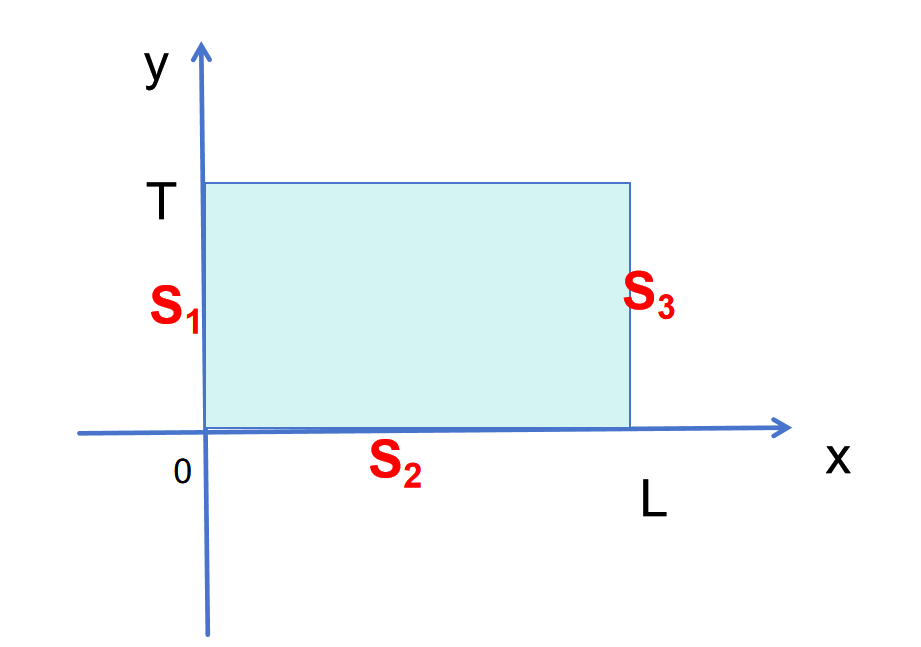
\includegraphics[width=10cm]{1.png}
	%\caption{售猪问题的净收益$f(x)$关于售猪时间$x$的曲线图}
\end{figure}

\textbf{定理1 (极值原理):} 假设函数 $ u=u(x, t) \in C^{2,1}(Q) \cap C(\overline{Q}) $ 且满足方程 (1), 那么 $ u(x, t) $ 在 $ \overline{Q} $ 上的最大值和最小值在边界 $ \Gamma $ 上可以达到, 即
$$
\max _{\overline{Q}} u(x, t)=\max _{\Gamma} u(x, t), \quad \min _{\overline{Q}} u(x, t)=\min _{\Gamma} u(x, t) .
$$

下面利用极值原理来讨论热传导方程解的唯一性和对边界及初始数据的连续依赖性 (即稳定性).

\textbf{定理2 :}初边值问题
\begin{equation*}
    \left\{\begin{array}{ll}
u_{t}=c^{2} u_{x x}+h(x, t), & 0<x<L, t>0, \\
u(x, 0)=f(x), & 0 \leqslant x \leqslant L, \\
u(0, t)=p(t), u(L, t)=q(t), & t \geqslant 0
\end{array}\right.\tag{2}
\end{equation*}
在函数空间 $ C^{2,1}(Q) \cap C(\overline{Q}) $ 中的解是唯一的, 且连续依赖初始和边界数据.

证: 先证解的唯一性. 设 $ u_{1}(x, t) $ 和 $ u_{2}(x, t) $ 是问题 (2) 在函数空间 $ C^{2,1}(Q) \cap C(\overline{Q}) $ 中的两个解. 记 $ u(x, t)=u_{1}(x, t)-u_{2}(x, t) $, 那么 $ u=u(x, t) $ 满足齐次方程和齐次初边值条件的定解问题
$$
\left\{\begin{array}{ll}
u_{t}=c^{2} u_{x x}, & 0<x<L, t>0, \\
u(x, 0)=0, & 0 \leqslant x \leqslant L, \\
u(0, t)=u(L, t)=0, & t \geqslant 0 .
\end{array}\right.
$$
对任意一点 $ \left(x_{0}, t_{0}\right), 0 \leqslant x_{0} \leqslant L, t_{0}>0 $, 记
$$
Q=\left\{(x, t) \mid 0 \leqslant x \leqslant L, 0 \leqslant t<t_{0}\right\}
$$
和 $ \Gamma $ 为 $ Q $ 的抛物边界. 那么 $ u(x, t) $ 在 $ \overline{Q} $ 上连续, 且满足
$$
u_{t}=c^{2} u_{x x}, \quad 0<x<L, 0<t \leqslant t_{0} .
$$
由定理 1 得, 对任意 $ (x, t) \in \overline{Q} $, 成立
$$
0=\min _{\Gamma} u(x, t) \leqslant u(x, t) \leqslant \max _{\overline{Q}} u(x, t)=0 .
$$
即在区域 $ \overline{Q} $ 上, $ u(x, t)=0 $. 特别地, $ u\left(x_{0}, t_{0}\right)=0 $ 和 $ u_{1}\left(x_{0}, t_{0}\right)=u_{2}\left(x_{0}, t_{0}\right) $. 由于 $ \left(x_{0}, t_{0}\right) $ 是任意的, 所以
$$
u_{1}(x, t)=u_{2}(x, t), \quad 0 \leqslant x \leqslant L, t \geqslant 0,
$$
这表明解是唯一的.

下面考虑解对初始数据和边界数据的连续依赖性. 设 $ u_{i}(x, t)(i=1,2) $ 是问题
$$
\left\{\begin{array}{ll}
u_{t}=c^{2} u_{x x}+h(x, t), & 0<x<L, t>0, \\
u(x, 0)=f_{i}(x), & 0 \leqslant x \leqslant L, \\
u(0, t)=p_{i}(t), u(L, t)=q_{i}(t), & t \geqslant 0
\end{array}\right.
$$
的解. 令 $ u(x, t)=u_{1}(x, t)-u_{2}(x, t), p(t)=p_{1}(t)-p_{2}(t), q(t)=q_{1}(t)-q_{2}(t) $, $ f(x)=f_{1}(x)-f_{2}(x) $. 则 $ u=u(x, t) $ 满足
$$
\left\{\begin{array}{ll}
u_{t}=c^{2} u_{x x}, & 0<x<L, t>0, \\
u(x, 0)=f(x), & 0 \leqslant x \leqslant L, \\
u(0, t)=p(t), u(L, t)=q(t), & t \geqslant 0 .
\end{array}\right.
$$
当 $ 0 \leqslant x \leqslant L, t \geqslant 0 $ 时, 如果有 $ |f(x)|<\varepsilon,|p(t)|<\varepsilon,|q(t)|<\varepsilon $, 那么由极值原理得 $ |u(x, t)|<\varepsilon, 0 \leqslant x \leqslant L, t \geqslant 0 $. 这就证明了初边值问题 (2) 解关于初始数据和边界数据的稳定性. 定理证毕.



\subsubsection{拉普拉斯方程的极值原理}
\textbf{定理: (极值原理) }$ \quad $ 设 $ \Omega $ 是 $ \mathbb{R}^{3} $ 中的有界区域, 边界 $ \partial \Omega $ 光滑. 如果 $ u \in $ $ C^{2}(\Omega) \cap C(\overline{\Omega}) $ 且满足
$$
\Delta u=u_{x x}+u_{y y}+u_{z z}=0, \quad(x, y, z) \in \Omega,
$$
则 $ u $ 在边界 $ \partial \Omega $ 上达到 $ \overline{\Omega} $ 上的最大值和最小值, 即
$$
\max _{\overline{\Omega}} u(x, y, z)=\max _{\partial \Omega} u(x, y, z), \quad \min _{\overline{\Omega}} u(x, y, z)=\min _{\partial \Omega} u(x, y, z)
$$
注. 设 $ u \in C^{2}(\Omega) $, 且 $ \Delta u>0 $ (或 $ \Delta u<0 $ ), 则 $ u $ 不可能在 $ \Omega $ 内达到最大 (最小) 值.


下面利用极值原理来讨论调和方程的第一边值问题解的唯一性和稳定性.

 设 $ \Omega $ 是 $ \mathbb{R}^{3} $ 中的一有界区域, 其边界 $ \partial \Omega $ 光滑. 如果泊松方程的狄利克雷内问题
$$
(1)\left\{\begin{array}{ll}
\Delta u=g(x, y, z), & (x, y, z) \in \Omega \\
u(x, y, z)=f(x, y, z), & (x, y, z) \in \partial \Omega
\end{array}\right.
$$
在函数空间 $ C^{2}(\Omega) \cap C(\overline{\Omega}) $ 中存在解, 则必唯一, 且连续依赖于边界数据.

证: 设 $ u_{1}, u_{2} $ 是问题 $ (1) $ 的两个解, 那么函数 $ u=u_{1}-u_{2} $ 满足
$$
\Delta u=0, \quad(x, y, z) \in \Omega ; \quad u(x, y, z)=0, \quad(x, y, z) \in \partial \Omega .
$$
由定理, 
$$
\max _{ \overline{\Omega}} u=\max _{ \partial \Omega} u=0, \quad \min _{ \overline{\Omega}} u=\min _{ \partial \Omega} u=0
$$
所以在 $ \Omega $ 内有 $ u=0 $, 即 $ u_{1}=u_{2} $.所以问题 (1) 的解是唯一的.
(注意到这里的 $ \Omega $ 是一个有界区域. 无界域上的边值问题, 解的唯一性不一定是对的. )

下面证明解对边界数据的稳定性.
设 $ u_{1} $ 和 $ u_{2} $ 是定解问题 (1) 分别对应于边值 $ f_{1} $ 和 $ f_{2} $ 的两个解, 则函数 $ u=u_{1}-u_{2} $ 满足
$$
\left\{\begin{array}{ll}
\Delta u=0, & (x, y, z) \in \Omega, \\
u(x, y, z)=f(x, y, z), & (x, y, z) \in \partial \Omega,
\end{array}\right.
$$
其中 $ f(x, y, z)=f_{1}(x, y, z)-f_{2}(x, y, z) $.
假定在边界 $ \partial \Omega $ 上, $ |f(x, y, z)|<\varepsilon $, 那么由定理 , 对任意 $ (x, y, z) \in \Omega $, 成立
$$
-\varepsilon<\min _{\partial \Omega}\left(f_{1}-f_{2}\right)=\min _{\partial \Omega} u \leqslant u(x, y, z) \leqslant \max _{\partial \Omega} u=\max _{\partial \Omega}\left(f_{1}-f_{2}\right)<\varepsilon .
$$
即对任意 $ (x, y, z) \in \bar{\Omega},|u(x, y, z)|<\varepsilon $. 所以定解问题 (1) 的解连续依赖于所给的边界数据. 证毕.
\subsection{热传导方程的柯西问题}
\subsubsection{齐次方程}

一维热传导方程的 Cauchy 问题是
\begin{equation*}
    u_{t}-a^{2} u_{x x}=0,-\infty<x<+\infty, t>0,\tag{1}
\end{equation*}
具有初始条件
\begin{equation*}
   \left.u\right|_{t=0}=\varphi(x), \quad-\infty<x<+\infty . \tag{2}
\end{equation*}

它的求解我们一般采用 Fourier 变换方法,在这里我们利用无量纲法推导出热传导方程的自相似解,然后我们将应用相似变换法求解 Cauchy 问题 (1), (2). 为此, 我们首先给出热传导方程 (1) 的解的如下性质. 这里就不提供证明.

性质 1. 设 $ u(x, t) $ 是 (1) 的解, 则对任意的 $ y \in \mathbf{R}, u(x-y, t) $ 也是 (1) 的解.

性质 2. 设 $ u(x, t) $ 是 (1) 的解, 则它的各阶导数 (比如 $ u_{x}, u_{t}, u_{x t}, u_{x x} $ 等) 也是 (1) 的解.

性质 3. 设 $ S(x, t) $ 是  (1) 的解, 则对任意连续函数 $ g(y) $,
$$
v(x, t)=\int_{-\infty}^{\infty} S(x-y, t) g(y) \mathrm{d} y
$$
也是 (1) 的解.
性质4. 设 $ u(x, t) $ 是 (1) 的解, 则对任意的 $ \lambda>0, u\left(\lambda x, \lambda^{2} t\right) $ 也是 (1) 的解.

由性质4 , 我们易知方程 (1) 具有如下形式的自相似解:
$$
Q(x, t)=q(\xi), \quad \xi=\frac{x}{\sqrt{t}} .
$$
经过简单的计算可知 $ q(\xi) $ 满足如下常微分方程
$$
q^{\prime \prime}+\frac{1}{2 a^{2}} \xi q^{\prime}=0
$$
其通解可通过两次积分求出:
$$
q(\xi)=c_{1} \int_{0}^{\xi} \mathrm{e}^{-\frac{1}{4 a^{2}} \eta^{2}} \mathrm{~d} \eta+c_{2},
$$
其中 $ c_{1}, c_{2} $ 是两个积分常数.
因此
$$
Q(x, t)=c_{1} \int_{0}^{\frac{x}{\sqrt{t}}} \mathrm{e}^{-\frac{1}{4 a^{2}} \eta^{2}} \mathrm{~d} \eta+c_{2}
$$
由性质2 知
$$
S(x, t)=\frac{\partial}{\partial x} Q(x, t)=\frac{c_{1}}{\sqrt{t}} \mathrm{e}^{-\frac{x^{2}}{4 a^{2} t}}
$$
是 (1) 的解, 从而由性质 3 知对任意连续函数 $ g(y) $
\begin{equation*}
    v(x, t)=\int_{-\infty}^{\infty} S(x-y, t) g(y) \mathrm{d} y=\frac{c_{1}}{\sqrt{t}} \int_{-\infty}^{\infty} \mathrm{e}^{-\frac{(x-y)^{2}}{4 a^{2} t}} g(y) \mathrm{d} y\tag{3}
\end{equation*}
也是 (1) 的解. 为了求出 Cauchy 问题 (1), (2) 的解, 我们利用初始条件 (2)确定 (3) 中的常数 $ c_{1} $.
事实上,作变换 $ y=x+2 a \sqrt{t} \eta $, 则 (3) 可改写为
$$
v(x, t)=2 a c_{1} \int_{-\infty}^{\infty} \mathrm{e}^{-\eta^{2}} g(x+2 a \sqrt{t} \eta) \mathrm{d} \eta .
$$
在该式中令 $ t \rightarrow 0^{+} $, 得
$$
\varphi(x)=v(x, 0)=2 a c_{1} \int_{-\infty}^{\infty} \mathrm{e}^{-\eta^{2}} g(x) \mathrm{d} \eta=2 \sqrt{\pi} a c_{1} g(x)
$$
因此,要使 (3)满足初始条件 (2), 必须取
$$
c_{1}=\frac{\varphi(x)}{2 \sqrt{\pi} \operatorname{ag}(x)} .
$$

将 $c_1$ 代人到 (3), 我们得到 Cauchy 问题 (1), (2) 的解为
\begin{equation*}
    u(x, t)=\frac{1}{2 a \sqrt{\pi t}} \int_{-\infty}^{\infty} \mathrm{e}^{-\frac{( x-y)^{2}}{4 a^{2} t}} \varphi(y) \mathrm{d} y .\tag{4}
\end{equation*}
我们通常称 (4) 为 Poisson 公式, 若记
$$
G(x, t)=\left\{\begin{array}{ll}
\frac{1}{2 a \sqrt{\pi t}} \mathrm{e}^{-\frac{x^{2}}{4 a^{2} t},} & t>0, \\
0, & t<0,
\end{array}\right.
$$
那么 (4) 可改写成
$$
u(x, t)=\int_{-\infty}^{\infty} G(x-y, t) \varphi(y) \mathrm{d} y .
$$
由其所确定的函数通常称为热核函数.(当然, 上面的推导完全是形式的.)

\subsubsection{非齐次方程}

我们考虑非齐次热传导方程的 Cauchy 问题
\begin{equation*}
    \left\{\begin{array}{ll}
u_{t}-a^{2} u_{x x}=f(x, t), & -\infty<x<+\infty, t>0, \\
\left.u\right|_{t=0}=\varphi(x), & -\infty<x<+\infty .
\end{array}\right.\tag{1}
\end{equation*}
由线性方程的叠加原理, (1) 的求解可分解为如下两个问题的求解
\begin{equation*}
\left\{\begin{array}{ll}
u_{t}-a^{2} u_{x x}=0, & -\infty<x<+\infty, \\
\left.u\right|_{t=0}=\varphi(x), & -\infty<x<+\infty,
\end{array}\right.\tag{2}
\end{equation*}
及
\begin{equation*}
\left\{\begin{array}{ll}
u_{t}-a^{2} u_{x x}=f(x, t), & -\infty<x<+\infty, t>0, \\
\left.u\right|_{t=0}=0, & -\infty<x<+\infty .
\end{array}\right.\tag{3}
\end{equation*}
即若 $ u_{1}(x, t), u_{2}(x, t) $ 分别是 Cauchy 问题 (2), (3) 的解, 则 $ u(x, t)=u_{1}(x, t) $ $ +u_{2}(x, t) $ 是 Cauchy 问题 (1) 的解.

Cauchy 问题 (2)的求解我们已经讨论过.下面我们用关于求解非齐次波动方程的 Duhamel 原理的方法来求解 Cauchy 问题 (3).

\textbf{引理(齐次化原理) }若函数 $ w(x, t, \tau) $ 是 Cauchy 问题
\begin{equation*}
\left\{\begin{array}{ll}
w_{t}-a^{2} w_{x x}=0, & -\infty<x<+\infty, \\
\left.w\right|_{t=r}=f(x, \tau), & -\infty<x<+\infty
\end{array}\right.\tag{4}
\end{equation*}
的解, 则函数
$$
u(x, t)=\int_{0}^{t} w(x, t, \tau) \mathrm{d} \tau
$$
就是 Cauchy 问题(3)的解.

为了应用 Poisson 公式 求解 Cauchy 问题 (4), 令 $ t^{\prime}=t-\tau $, 得如下 Cauchy 问题:
$$
\left\{\begin{array}{l}
w_{t^{\prime}}-a^{2} w_{x x}=0, \quad-\infty<x<+\infty, t^{\prime}>0 \\
\left.w\right|_{t^{\prime}=0}=f(x, \tau), \quad-\infty<x<+\infty .
\end{array}\right.
$$
易知解为
$$
w\left(x, t^{\prime}, \tau\right)=\int_{-\infty}^{\infty}=G\left(x-y, t^{\prime}\right) f(y, \tau) \mathrm{d} y .
$$
从而 (4) 的解为
\begin{equation*}
w(x, t, \tau)=\int_{-\infty}^{\infty} G(x-y, t-\tau) f(y, \tau) \mathrm{d} y .\tag{5}
\end{equation*}

由引理及 (5), 我们能获得 Cauchy 问题 (1) 的解:
$$
u(x, t)=\int_{-\infty}^{\infty} G(x-y, t) \varphi(y) \mathrm{d} y+\int_{0}^{t} \int_{-\infty}^{\infty} G(x-y, t-\tau) f(y, \tau) \mathrm{d} y \mathrm{~d} \tau .
$$

\subsection{二阶线性方程的分类}
含两个自变量的二阶线性偏微分方程的一般形式是
$$
a_{11} u_{x x}+2 a_{12} u_{x y}+a_{22} u_{y y}+b_{1} u_{x}+b_{2} u_{y}+c u=f
$$
其中 $ a_{11}, a_{12}, a_{22} $ 不同时为零. 方程的分类依赖于行列式 $ \Delta=a_{11} a_{22}-a_{12}^{2} $ 的取值或矩阵 $ A=\left(\begin{array}{ll}a_{11} & a_{12} \\ a_{21} & a_{22}\end{array}\right) $ 的特征值 $ \lambda_{1}, \lambda_{2} $ 的符号.

若 $ \Delta>0 $ (等价地, $ \lambda_{1}, \lambda_{2} $ 不等于零且同号), 则称方程 为椭圆型的;

若 $ \Delta<0 $ (等价地, $ \lambda_{1}, \lambda_{2} $ 不等于零且异号), 则称方程 为双曲型的;

若 $ \Delta=0 $ (等价地, $ \lambda_{1}, \lambda_{2} $ 有一个为零), 则称方程  为抛物型的.